\documentclass[5p]{elsarticle}
%\documentclass[aps,prb,twocolumn,showpacs,floatfix,superscriptaddress]{revtex4}
\usepackage{lineno,hyperref}
\usepackage{epsfig,amsmath,amssymb, mathrsfs,psfrag}
\modulolinenumbers[5]

\usepackage{graphicx}
\usepackage{caption}
\usepackage{subcaption}
\usepackage[]{algorithm2e}

%%%%%%%%%%%%%%%%%%%%%%%
%% Elsevier bibliography styles
%%%%%%%%%%%%%%%%%%%%%%%
%% To change the style, put a % in front of the second line of the current style and
%% remove the % from the second line of the style you would like to use.
%%%%%%%%%%%%%%%%%%%%%%%

%% Numbered
\bibliographystyle{model1-num-names}

%% Numbered without titles
%\bibliographystyle{model1a-num-names}

%% Harvard
%\bibliographystyle{model2-names.bst}\biboptions{authoryear}

%% Vancouver numbered
%\usepackage{numcompress}\bibliographystyle{model3-num-names}

%% Vancouver name/year
%\usepackage{numcompress}\bibliographystyle{model4-names}\biboptions{authoryear}

%% APA style
%\bibliographystyle{model5-names}\biboptions{authoryear}

%% AMA style
%\usepackage{numcompress}\bibliographystyle{model6-num-names}

%% `Elsevier LaTeX' style
%\bibliographystyle{elsarticle-num}
%%%%%%%%%%%%%%%%%%%%%%%

\begin{document}

\begin{frontmatter}

\title{Meanfield theory of activation functions in Deep Neural Networks}

%% Group authors per affiliation:
 \author[mirco]{Mirco Milletar\'i\corref{cor} \fnref{fn1}}
    \ead{milletari@gmail.com}

 \author[thip]{Thiparat Chotibut }
    \ead{thiparatc@gmail.com}

 \author[paolo]{Paolo E. Trevisanutto}
 \ead{pe.trevisanutto@nus.edu.sg}


\fntext[fn1]{This work was initiated while in Bambu.}
\cortext[cor] {Corresponding Author}

\address[mirco]{Microsoft, Singapore}
\address[thip]{Singapore University of Technology and Design, Singapore.}
\address[paolo]{Graphene Research Centre and CA2DM, National University of Singapore, Singapore. }


\begin{abstract}
We present a statistical mechanics model of deep neural networks, connecting the energy-based and the feed forward (FFN) approach.
We infer that FFN can be understood as performing three basic steps: {\it encoding}, { \it representation validation} and {\it propagation}. From the meanfield solution of the model, we obtain a set of natural activations -- such as {\it sigmoid}, $\tanh$ and {\it ReLU} -- together with a state-of-the-art one, recently introduced heuristically by Elfwig et al.~\cite{elfwig} and Ramachandran et al.~\cite{prajit}, \textit{Swish}. In this article, we show how \textit{Swish} can be obtained as a meanfield solution of our model for the expected information propagating through the network and show how this tends to \textit{ReLU} in the limit of zero noise. To the best of our knowledge, this also provides the first derivation of the \textit{ReLu} activation function.

Finally, we study the eigenvalue spectrum of the Hessian on an associated classification task, showing that \textit{Swish} acts as a natural regularizer and allows for faster training and more consistent performances over a wider range of network architectures.

\end{abstract}

\begin{keyword}

\end{keyword}

\end{frontmatter}

\linenumbers

\section{Introduction}

Advances in modern computing hardware and availability of massive datasets have empowered multilayer artificial neural networks, or deep learning, with unprecedented capabilities for image and speech recognition tasks. Despite these empirical success, theoretical understanding of why and when multilayer neural networks perform well lags far behind~\cite{mezard1}.
Only recently, theoretical efforts in this direction have been intensively reported. For example, recent works shed light on how FFN attains its expressive power~\cite{Poggio2017, LinTegmark2017, Raghu2017, Poole2016}, what contributes to its generalizability~\cite{Zhang2017,Dinh2017}, and how myriad parameters in the network affect the geometry of the loss function ~\cite{dauphin, ch, penn1, penn2}. Taken together, these theoretical results have paved the way for a systematic design of robust and explainable FFNs.

Although FFN is one of the most studied and widely used neural network architectures, state-of-the-art models still largely inherit their building blocks from the decades-old multilayer perceptron (MLP). By augmenting MLP with modern optimization techniques such as dropout~\cite{srivastava2014}, non-linear activation functions, and specialized complex network architectures~\cite{Krizhevsky}, to name a few, the FFN can be efficiently trained on large-scale datasets such as ImageNet or CIFAR to achieve low training and generalization errors.
While these engineering feats improve the performance of FFN, a clear design principle behind these developments is still lacking. This leads to an unsystematic growth of the FFN complexity, which obscures its original exposition as a simple physical system that can perform non-linear classification and regression tasks.


To assist future systematic studies and construction of FFNs,  we propose a theoretical framework based on the tool-set of statistical mechanics. It allows for the definition of an energy based model in which a hidden unit is regarded as a communication channel, first encoding and then {\it transmitting} the result of its computation through a gate with a specific transmission probability; as opposed to a hidden unit in multilayer perceptrons that transmits its sigmoidal firing probability, or in modern FFNs where a standard \textit{ad hoc} activation function such as {\it ReLU} and its variants are used. The transmission probability is obtained via the maximum entropy principle~\cite{zecchina, jaynes} under the biologically inspired constraint that a neuron responds by firing (transmit its signals) or not with a certain probability. The maximum entropy principle provides the least biased probabilistic interpretation of a hidden neuron, and recasts a FFN as an energy-based model.
By interpreting a hidden unit as a communication channel, its activation function takes the form of the expected (mean) signal transmission; remarkably, this activation function agrees with the state-of-the-art, activation ({\it Swish}), obtained in Ref.~\cite{prajit} through an extensive search algorithm trained with reinforcement learning and shown to best perform on the CIFAR and ImageNet datasets among all candidate activations. Although some of these activations may perform better for the specific datasets they have been built for, they generally fail to generalize. Finally, the standard {\it ReLU} activation arises as a limiting case of the {\it Swish}, corresponding to the noiseless limit of a communication channel. To the best of our knowledge, this provides the first formal derivation of the {\it ReLU} activation, typically introduced heuristically to facilitate optimization protocols. Despite restricting our analysis to pure FFNs, most of our conclusions carry on to Convolutional and Recurrent networks, which will be addressed in future works.


The paper is organized as follows:  In section 2, we provide a plausible argument based on dimensional analysis to explain why a hidden unit should be regarded as a communication channel transmitting the result of its computation. We then discuss the formulation of a FFN as an energy-based model using the maximum entropy principle over the binary states of a hidden unit, and discuss the advantage of this formulation. In analogy with Refs.~\cite{tishby1, tishby2}, we show that each hidden unit acts first as an encoder and then as a filter determining the quality of its input by comparing it with a local bias potential.

In section 3, we explore the geometry of loss surfaces associated with training FFNs with {\it Swish} hidden units on simple classification tasks. The index $\alpha$, representing the fraction of negative eigenvalues of the Hessian (a measure of the number of descent directions), as well as the index $\gamma$, representing the fraction of zero eigenvalues (a measure of the number of flat directions), are investigated. We find that FFNs trained with {\it ReLU} exhibit $\gamma \neq 0$  while those trained with {\it Swish} often show $\gamma \simeq 0$, resulting in faster and more flexible training. These two indices seem to determine not only the speed of learning but also whether learning will be successful, although further studies are required to understand the detailed dynamics of gradient descent. Lastly, we conclude by commenting on how our model relates (and incorporates) other recently proposed frameworks such as the Renormalization Group~\cite{mehta} and the information Bottleneck~\cite{tishby1, tishby2} in section 4. Codes and other numerical results, including training on the MNIST dataset, are provided in the appendix.

%
\section{Motivation and Model} \label{sec:model}

\subsection{General Setup} \label{sub:setup}

A standard task in supervised learning is to determine an input/output relation between a set of $m$ features and the observed labeled outcomes. Let us denote with $x^{\mu}_i$ the input vector, where $i \in [1, n]$ denotes a feature component, and $\mu \in [1,m]$ denotes an example; we also denote the output as $y^{\mu}_k$, where $k$ is the number of classes. Quite generally, the probability of measuring the output $\mathbf{y}$ given the input can be written as
%
\begin{align} \label{eq:chain} \nonumber
P(\mathbf{y}) &= \int d\mathbf{x} \, P(\mathbf{y} | \mathbf{x}) \, P(\mathbf{x}) =   \int d \hat{\mathbf{y}}\,  P(\mathbf{y} | \hat{\mathbf{y}} ) \int d \mathbf{j}   \, P(\hat{\mathbf{y}}| \mathbf{j} )   \\
&\times \int d \mathbf{x} \, P(\mathbf{j} | \mathbf{x} ) \, P(\mathbf{x}) =  \int d \hat{\mathbf{y}} \, P(\mathbf{y} | \hat{\mathbf{y}} ) \, P(\hat{\mathbf{y}}),
\end{align}
%
 where we have introduced the output of the outmost hidden layer ($\hat{ \mathbf{y}}$) and the output information of the hidden units  ($\mathbf{j}$); additional hidden layers can be introduced by further use of the chain rule. In exchanging the order of the integrals we have assumed that the probabilities are analytic functions of theory arguments. Once $P(\hat{\mathbf{y}})$ has been learned, one can obtain the loss function by taking the log-likelihood $\mathscr{L} = - \log P(\mathbf{y})$; for example, if we are considering a binary classification problem, $P(\hat{\mathbf{y}}[\boldsymbol{\theta}])$ is a Bernoulli distribution parametrized by a set of parameters $\boldsymbol{\theta_l} = \{\mathbf{W}_l,\mathbf{ b}_l \}$, being the weights and biases of the neural network, with $l \in [1, L]$ the number of hidden layers. In this case, the loss function corresponds to the binary cross-entropy but other statistical assumptions lead to different Losses; In \eqref{a:loss} we provide a derivation of the cross-entropy loss function using mean-field theory and highlights some of the assumptions underlying the result. To motivate the model, in the next section we begin by discussing a (physical) dimensional inconsistency in the standard formulation of {\it forward propagation} in FFNs, and how this can be reconciled within the proposed framework. With some terminology borrowed from physics jargon, in the following text we use the term ``physical dimension''  (or simply ``dimension'') to denote the unit used to measure a variable, e.g. the dimension of length is, in SI units, metre.

\begin{figure*}[t!]
 \centering
  	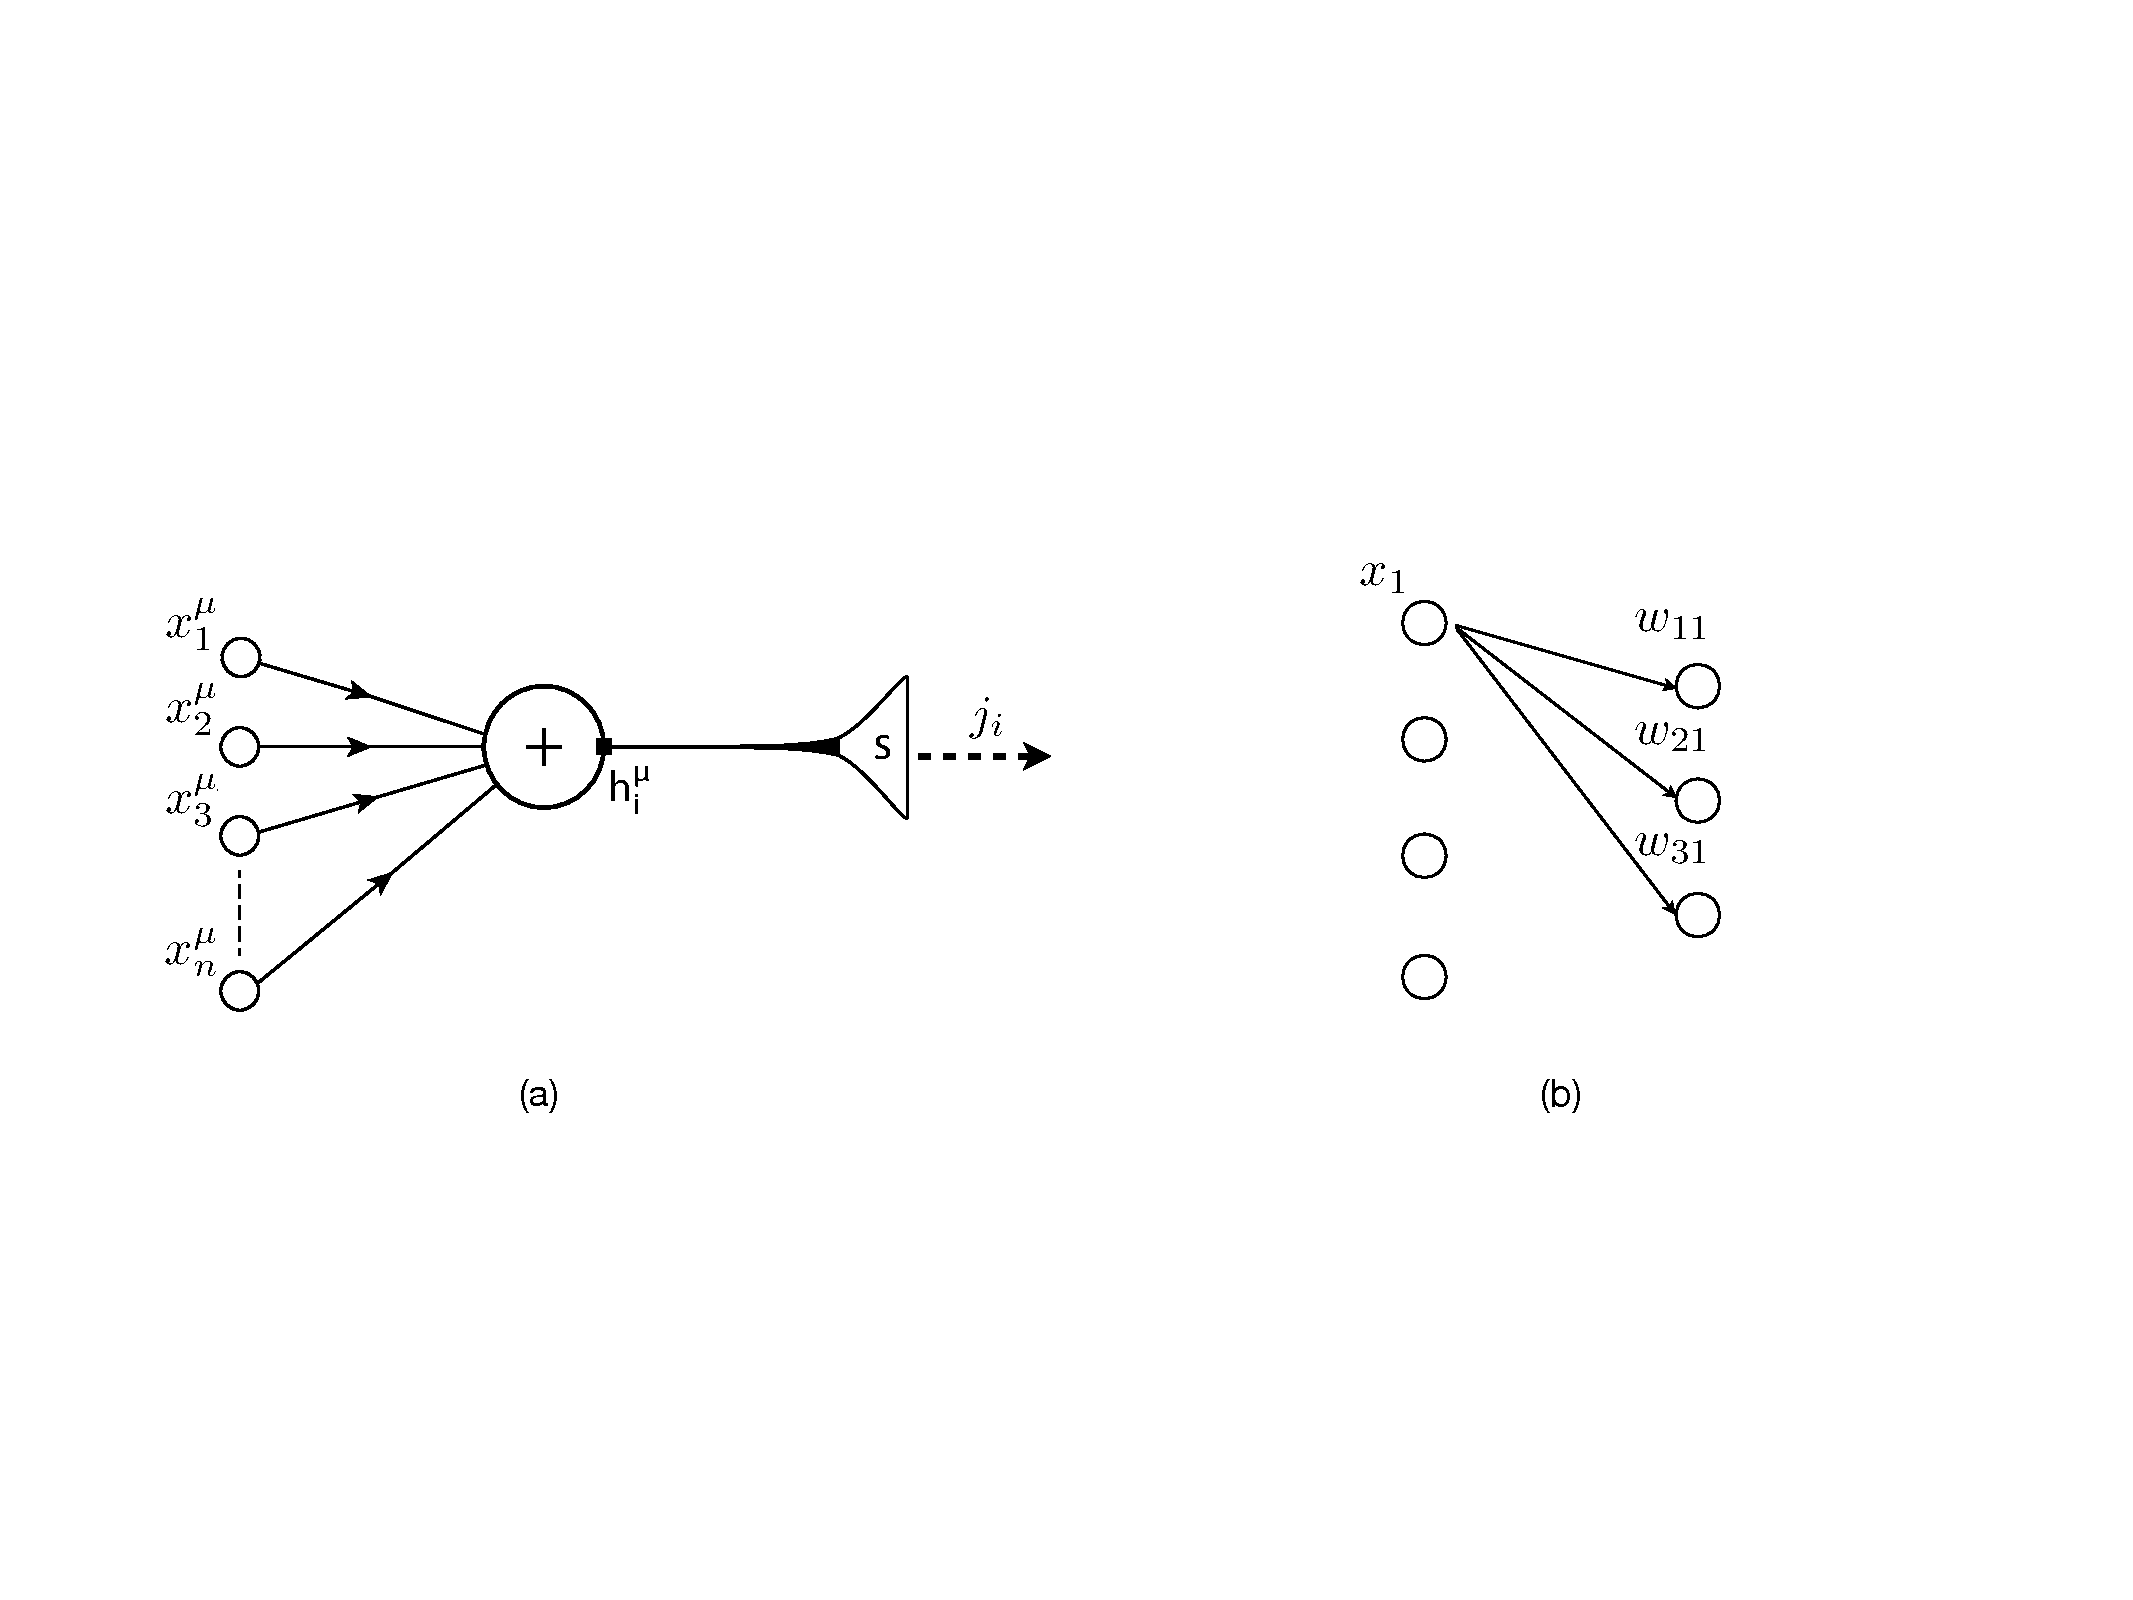
\includegraphics[width = .8\textwidth]{fig1.pdf}
  	\caption{(a) Schematic representation of a neuron in an artificial neural network. The empirical input $x^{\mu}_i$ is processed to give a new representation $h^{\mu}_i$. For a compression layer, this is obtained by taking a linear combination of the input. The signal $h_i$ goes through the ``synaptic'' gate $s_i$ that can be either open or close given the signal exceeding a threshold potential $b$ (this is included in the definition of $h_i$ for convenience). The output signal $j_i = h_i \, s_i$ is zero if $s_i=0$ or equal to the processed information $h_i$ if it is open. (b) Information conservation between different layers.  In the example above, the input $x_1$ is ``fractionalized'' in the units of the next layer. Information conservation simply demands that $w_{11} x_1 + w_{21} x_1 + w_{31} x_1 = x_1$, hence $\sum_i w_{i1}=1$. }
	\label{fig:synapse}
\end{figure*}

\subsection{Motivations} \label{sub:mot}
%
 Motivated by neurobiology and in analogy with the communication channel scheme in information theory~\cite{mckay, jaynes}, we regard the input vector $x^{\mu}_i$ as the information source entering the processing units (neurons) of the network, while the units constitute the encoders. Quite generally, the encoders can either build a lower (compression) or higher dimensional (redundant) representation of the input data by means of a properly defined transition function. In a FFN, the former corresponds to a compression layer (fewer units) while the latter to an expansion layer (more units). If the encoded information constitutes an informative representation of the output signal (given the input), it is passed  over to the next layer for further processing until the output layer is reached. In the biological neuron, this last step is accomplished by the synaptic bouton, that releases information whether or not the input signal exceeds a local bias potential $b_i$, see Fig.~\eqref{fig:synapse} for a schematic representation. Both in the brain and in electronic devices, the input information is often conveyed in the form of an electric signal, with the electron charge being the basic unit of information, the signal has dimension (units) of $Coulomb$ in SI. For an image, the information is the brightness level of each pixel, physically proportional to the current passing through it; on a computer, this is encoded in bits. Clearly, a linear combination of the input signals, together with the bias, has to preserve dimensions:
%
\begin{equation} \label{eq:lincomb}
h^{\mu}_i = \sum_{j=1}^{n} \, w_{ij} x^{\mu}_j + b_i,
\end{equation}
%
where $i \in [1, n_1]$ indices the receiving units in the first layer and the weight matrix $ w_{ij}$ is the coefficient of the linear combination and it is dimensionless.

For noiseless systems, the input signal is transmitted i.f.f. the overall signal exceeds the bias $b_i$. However, in the presence of noise, the signal can be transmitted with a certain probability even below the threshold; in the biological neuron, the variance in the number of discharged vesicles in the synaptic bouton and the number of neurotransmitters in each vesicle is responsible for the noisy, asynchronous dynamics~\cite{amit1}. In so far, we just described the general functioning principle underlying FFNs. Let us first consider the sigmoid non-linearity $\sigma(\beta \, \mathbf{h} )$, where $\beta$  has inverse dimension of $\mathbf{h}$;  $\sigma$ expresses the probability of the binary unit to be active (1) and can be seen as an approximation of the biological neuron's firing probability~\cite{amit1}. Being a {\it distribution function} defined in $[0,1]$, $\sigma$ is intrinsically {\it dimensionless}. The parameter $\beta$ defines the spread of the distribution, tuning to the noise strength; typically, one sets $\beta =1$ or reabsorb it inside the weights and bias~\cite{zecchina}, but here we keep it general for reasons that will be clear later. Defining $\mathbf{a} = \sigma(\beta \, \mathbf{h} )$ as the input of the next layer, we can immediately see the dimensional mismatch: a linear combination of $\mathbf{a}$ is dimensionless and when passed through the new non-linearity, $\sigma(\beta \, \mathbf{a} )$ necessarily becomes dimensionful ($\beta \, \mathbf{a}$ now has dimension of noise). In the next section we show how this simple fact is at the root of the well known phenomena of vanishing gradients during back propagation. From a conceptual point of view, one is transmitting the expectation value of the transmission gate (synapse) rather than the processed signal. This problem persists when using the $\tanh$ activation (a translation of the sigmoid), but it is absent when using {\it ReLU}, that correctly transmits the information itself. In the next subsection we formalise this intuitive picture using the tools of statistical mechanics.

\subsection{Statistical mechanics of Feed Forward networks}

A prototypical statistical mechanics formulation of Neural Networks is the {\it inverse} Ising problem~\cite{zecchina}, where one is interested in infering the values of the couplings and external fields of the Ising model, given a set of pairwise connected binary units $s_i$; in computer science, this problem is solved by the Boltzmann machine. While the Boltzmann machine is an energy-based model, standard FFN is not commonly regarded as such. Here, we propose an energy-based formulation of FFNs to bridge on these two formulations, solely based on the maximum entropy principle ~\cite{zecchina, roberto, mckay, jaynes} to obtain the least biased probabilistic interpretation of hidden neurons. Eq.~\eqref{eq:chain} describes the general structure of the network, in the following we link this structure to a model of artificial neurons qualitatively described in section~\eqref{sub:mot} and depicted in Fig.~\eqref{fig:synapse}. Starting from the input layer, each unit takes the same input vector $\mathbf{x}$ and processed to output a new variable $\mathbf{h}$.
	One of the central results of this paper is based on the identification of $h_i$ as an effective, coarse grained field coupling to the synaptic gate variable $s_i$~\footnote{ Here we refer to compression layers, but similar conclusions hold for expansion ones.}. The feedforward nature of coarse graining (a directed graph), stems from the fact that it is not possible to entirely retrieve the original information after eliminating part of it; this endorses the forward pass with a semi-group structure. Considering the first layer, we need to evaluate the probability associated to the new, coarse grained variable $\mathbf{h}$,
%
\begin{equation} \label{eq:ps1}
P(\mathbf{h}) =  \int d \mathbf{x} \, Q(\mathbf{h} | \mathbf{x} ) \, P(\mathbf{x}),
\end{equation}
%
where  $Q(\mathbf{h} | \mathbf{x} )$ is the transition function modelling the encoder. In deep learning, the form of the transition function is fixed by the forward pass operation, while the  input data are drawn from some unknown distribution $P(\mathbf{x})$. We can follow two different paths: fix the value of $\mathbf{x}$ on the observed (empirical) sequence, or assume the form of the distribution from which $\mathbf{x}$ has been sampled from. The former corresponds to an empirical dataset, whereas the latter is preferred for an analytical inspection and to determine general statistical properties about the system. In this work we consider the former, while the latter will be discussed in a forthcoming manuscript. Consider then the empirical estimator $P(\mathbf{x}) =  \prod_{\mu=1}^m  \delta( \mathbf{x} - \mathbf{x}^{\mu} )$, where the Dirac-delta function is a representation of an indicator function, fixing the input on the observed sequence $x_i^{\mu}$. As for the transition function, it enforces the information processing performed by the ``soma'' of the artificial neuron; in the
	case of Deep Learning this consists in creating a linear combination of the input information. As information needs to be conserved, an additional constrain should be imposed on the coefficients of the transformation, namely $\sum_i \, w_{ij}^{[l]} =1$ $\forall l = 1, ..., L$, see Fig.~\eqref{fig:synapse} for an explicit example. It is interesting to note that this constraint is equivalent to the conservation of charge in an electronic system and to an $L_1$-type regularisation in machine learning.
%
\begin{align} \label{eq:ps2}
P(\mathbf{h}) &= \int {d\mathbf{x}} \, \Gamma^{[1]} \, \delta\left( \mathbf{h} -  \mathbf{w}^{T} \, \mathbf{x} - \mathbf{b} \right) \prod_{\mu =1}^m  \delta ( \mathbf{x} - \mathbf{x}^{\mu} )  \\ \nonumber
&= \frac{\Gamma^{[1]}}{m} \sum_{\mu}  \delta \left( \mathbf{h} -  \mathbf{w}^{T} \, \mathbf{x}^{\mu} - \mathbf{b} \right) \\
\Gamma^{[1]} &= \prod_{j=1}^n \delta\left( \sum_{i=1}^{n_1} w_{ij}^{[1]} -1 \right) .
\end{align}
%
Eq.~\eqref{eq:ps2} can be interpreted in different ways: it is akin to the real space block-spin renormalization developed by Kadanoff, reformulated in the more general language of probability theory~\cite{roberto, ma, cassandro} or it can be seen as a way to implement a ``change of variables'' from $x$ to $h$. The relation between Deep Learning and the renormalization group (RG) was previously observed in the context of restricted Boltzmann machine~\cite{mehta} and we now show that this connection holds here as well. Consider Eq.~\eqref{eq:ps2}, using the Fourier representation of the Dirac-delta function and performing the first integral over $\mathbf{x}$ we obtain
%
\begin{align} \label{eq:rbm}
P(\mathbf{h}) =\int_{-i \infty}^{i \infty} \frac{d\boldsymbol{\phi}  \,  \Gamma^{[1]} }{\sqrt{2\pi \, i}} e^{-\sum_{i} \phi_i \, h_i } e^{\frac{1}{m} \sum_{\mu} \sum_{ij} \phi_i \, w_{ij}^{[1]} x_{j}^{\mu} +\sum_i \phi_i \, b_i ^{[1]}  }.
\end{align}
 %
The second exponential is the RBM, with $x_i^{\mu}$ the visible units fixed on the data and $\phi_i$ a set of continuous valued  hidden units. The first exponential on the other hand asserts that $\phi$ and $h$ are dual variables. Before moving to the next step, we note in passing that while the discussion here and in Ref.~ \cite{mehta} suggests that feedforward propagation in the compression layer is analogous to the coarse graining step of RG, rescaling of the coarse grained variable is missing~\footnote{Alternatively, one can interpret $\mathbf{h}$ as an effective cavity field representing the action of units $s_i$ on unit $s_j$, see e.g. Ref.~\cite{parisi1} and \cite{opper} for connections to the belief propagation algorithm. }.

Once the coarse grained variables have been computed, the information passes through the ``synaptic'' gate that will transmit it with a certain probability if it exceeds the threshold potential $b_i$. The core task at hand is to determine the state of the gate (open/close). The absence of lateral connections in FFNs means that each synaptic gate is only influenced by its receptive signal, and the intralayer correlations are taken -- a priori-- to be zero. In other words, each unit within the same layer behaves independently of the others (i.e. no contextual information). Given a statistical ensemble of hidden binary gates, the most likely (and the least biased) distribution  can be obtained by maximising its entropy, subject to constraints imposed by the conserved quantities; in the grand canonical Gibbs ensemble these are the {\it global} average energy and particle number~\cite{roberto}, while here they correspond to the first and second moments of the data~\cite{zecchina, mckay}. However, in the absence of lateral connections, the entropy functional of the hidden gate $s_i$ does not account for the second moment and it reads
%
\begin{align} \label{eq:entropy2}
\mathscr{F} &= - \sum_{\mathbf{s}} P(\mathbf{s}) \, \log P(\mathbf{s}) + \eta \left( \sum_{\mathbf{s}} P(\mathbf{s}) -1\right) \\ \nonumber
&+ \sum_i \, \lambda_i \left( m_i -  \sum_{\mathbf{s}} \, s_i \, P(\mathbf{s}) \right),
 \end{align}
 %
where $\lambda_i$ are Lagrange multipliers chosen to reproduce the first moment of the data,  while $\eta$ enforces normalization. Functionally varying with respect to the probability $P(\mathbf{s)}$ and solving for the Lagrange multipliers, one  obtains~\cite{roberto}:
%
\begin{align} \label{eq:entropy4}
P(\mathbf{s} | \mathbf{h}) &= \frac{1}{Z} \, e^{ \sum_i \beta_i  \, s_i \, h_i } \\ \nonumber
Z[\mathbf{h}] &= \prod_i \, \sum_{s_i = \{ 0,1\} } e^{\beta_i \, s_i \, h_i}  =\prod_i \, \left( 1+ e^{\beta_i \, h_i} \right).
\end{align}
%
The parameters $\beta_i$ encode the noise, or statistical uncertainty of $s_i$ ($\lambda_i = \beta_i \, h_i$).  In a physical system, $\beta_i$ is the inverse temperature in units of Boltzmann's constant and in equilibrium it is the same for each $s_i$; however, here the network is only in a local equilibrium as the units are not allowed to exchange ``energy'' (information) among themselves due to the lack of pairwise interactions (the lateral connections)~\footnote{Technically, this corresponds to a generalized Gibbs ensemble, where conserved quantities are local rather than global, see e.g.~\cite{calabrese} }. We have also introduced the notation $P(\mathbf{s} | \mathbf{h})$ to denote the conditional probability of $\mathbf{s}$ given the signal $\mathbf{h}$ --  and the partition function $Z$.



Finally, given the distribution of the coarse grained inputs and the conditional probability of the channels $P(\mathbf{s}|\mathbf{h})$, one needs to evaluate the channel transmission probability
%
\begin{align} \label{eq:ps3}
P(\mathbf{s}) &= \int d \mathbf{h} \, P(\mathbf{s} | \mathbf{h}) \, P(\mathbf{h}) =  \frac{1}{Z} e^{-\sum_i \, \beta_i \mathscr{H}_i[s, x^{\mu}]}   \\ \nonumber
Z &= \frac{1}{m} \prod_{\mu=1}^m \prod_{i=1}^{n_1} \left[1+ e^{\beta_i \, h^{\mu}_i} \right] =\frac{1}{m} \prod_{\mu=1}^m \prod_{i=1}^{n_1} Z_{i, \mu},
\end{align}
%
where $\hat{h}^{\mu}_i = \sum_{j} w^{[1]}_{ij} \, x^{\mu}_j + b_i $,   $Z_{i, \mu}$ is the partition function per example/index and we have identified the simple coarse grained Hamiltonian
%
\begin{equation} \label{eq:Hamilton}
\mathscr{H}_i = -  \, \sum_{j=1}^n \, s_i \, w^{[1]}_{ij} x^{\mu}_j -  \, s_i \, b_i.
\end{equation}
%
Eqs.~\eqref{eq:ps3} and \eqref{eq:Hamilton} can be seen as the starting point of an {\it energy based model}, where it is the coarse grained probability $P(\mathbf{s})$ that propagates through the network (see e.g.~\cite{connie} ) as opposed to signals in a FFN; indeed, the above Hamiltonian has again the form of an RBM, this time with binary hidden units. The expected value of the channel transmission, $\langle s_i \rangle$ is~\cite{hertz}
%
\begin{equation} \label{eq:ps4}
\langle s_i \rangle = \frac{1}{\beta_i} \frac{\partial}{\partial b_i} \log Z_{i, \mu} =  \frac{1}{1+ e^{-\beta_i \, \hat{h}^{\mu}_i}} \equiv   \sigma(\beta_i \, \hat{h}^{\mu}_i),
\end{equation}
%
 the logistic function evaluated for each empirical realization $\mu$ and unit $i$. We stress that this quantity is not the coarse grained input signal {\it transmitted} by the channel; it solely determines the expectation of channel transmissions {\it given} the coarsed grained input signal $h_i^{\mu}$. Note that $\langle s_i \rangle$ would be the correct quantity for a single perceptron, or equivalently the output layer of an MLP performing a classification task. However, as discussed in the previous section, the hidden layers should not transmit $\langle s_i \rangle$, as this leads to dimensional mismatch.

 To ensure dimensional consistency across hidden layers, the output signal of each hidden unit must have the same dimension as its input signal. Therefore, the correct quantity to consider is the {\it expectation value} of the output signal $j_i = h_i \, s_i $, see  Fig.~\eqref{fig:synapse}.  This can be  obtained by summing over all gate states, for each unit and example, or by using the partition function of Eq.~\eqref{eq:ps3},
%
\begin{equation} \label{eq:ps5}
\langle j_i \rangle = \langle \hat{h}_i^{\mu} \, s_i \rangle_s = \frac{\partial}{\partial \beta_i} \log{Z_{i,\mu}} = \hat{h}^{\mu}_i \, \sigma(\beta_i \, \hat{h}^{\mu}_i),
\end{equation}
%
that agrees with the definition of the energy flux in statistical mechanics~\cite{bellac}. Note that contrary to Eq.~\eqref{eq:ps4}, the noise parameters $\beta_i$ cannot be rescaled away now.  This function was recently obtained in Ref.~\cite{prajit} (there named {\it Swish}), through an extensive search algorithm trained with reinforcement learning. In their extensive search, the authors found that activations of the form $a = x f(x)$  better performed on several benchmark datasets.
Now we interpret this activation function as an ``Expected Signal Propagation'' to stress its meaning and physical analogy, even though here $\beta$ does not have to be strictly positive.
        A theoretical study of the performance of {\it Swish} from the point of view of information propagation has been proposed in Ref.~\cite{soufiane}.  Our model naturally explains these studies by identifying {\it Swish} with the expectation value of the coarse grained input transmitted by each unit. In the next section we will better analyze {\it Swish} its meaning within backward propagation, and how it modifies the geometry of the loss surface.


Consider now the limit of a noiseless system, i.e. $\forall \, i$, $\beta_i \to \infty $ in the above equation:
%
\begin{equation} \label{eq:ps6}
\lim_{\beta_i \to \infty } \langle j_i \rangle =  \hat{h}^{\mu}_i \, \theta(\hat{h}^{\mu}_i)  \equiv   \rm{max} \left\{ \hat{h}^{\mu}_i, 0\right\} \equiv ReLU,
\end{equation}
%
where $\theta(.)$ is the Heaviside step function and in the last equality we have identified the {\it ReLU} activation. To the best of our knowledge, this is the first consistent derivation of {\it ReLU}, usually obtained following heuristic arguments. {\it ReLU} emerges as the noiseless limit of the mean transmitted information across the units; as such, it is not affected by the dimensional mismatch as it can be easily checked following the argument presented in Sec.~\eqref{sub:mot}. In Sec.~\eqref{sub:back} we discuss how the empirical observation that  {\it ReLU}  is not affected by the vanishing gradient problem is related to the absence of dimensional mismatch and the concept of expected signal propagation. We would like to stress that both {\it Swish} and {\it ReLU} pass on the expected value of their computation; the latter does it with probability one {\it only} if the coarse grained input signal exceeds a threshold, while the former can pass a signal lower than the threshold with a finite probability. In Fig.~\eqref{fig:activations} we plot the three activation functions for $\beta=1$. Clearly, {\it Swish} encompasses the statistical uncertainty conveyed by each processing unit in estimating the pre-activation value $h$. A positive value of the activation tells the units in the next layer that a certain combination of the previous inputs should be strengthen while a negative value means that it should be weakened, i.e. unlearned; the latter option is absent when using the {\it ReLU} function, a feature known to generally slow down learning~\cite{engel}. In the opposite extreme, the noisy limit $\beta \ll 1$, the {\it Swish} becomes linear. Therefore, we can consider linear networks as a noisy limit of non linear ones.
%
\begin{figure*}[t!]
    \centering
    \begin{subfigure}[b]{0.33 \textwidth}
        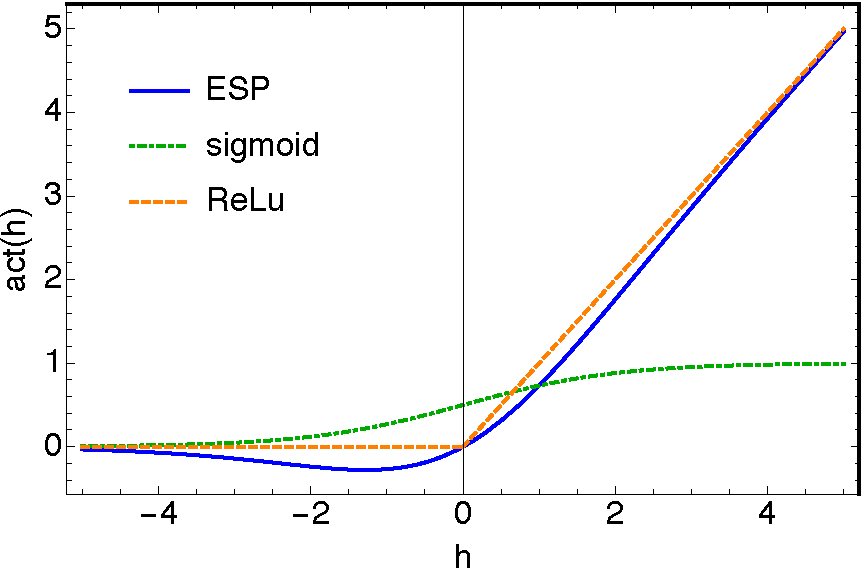
\includegraphics[width= \textwidth]{activations.pdf}
        \caption{activation}
        \label{fig:activation}
    \end{subfigure}
    ~
    \begin{subfigure}[b]{0.34 \textwidth}
        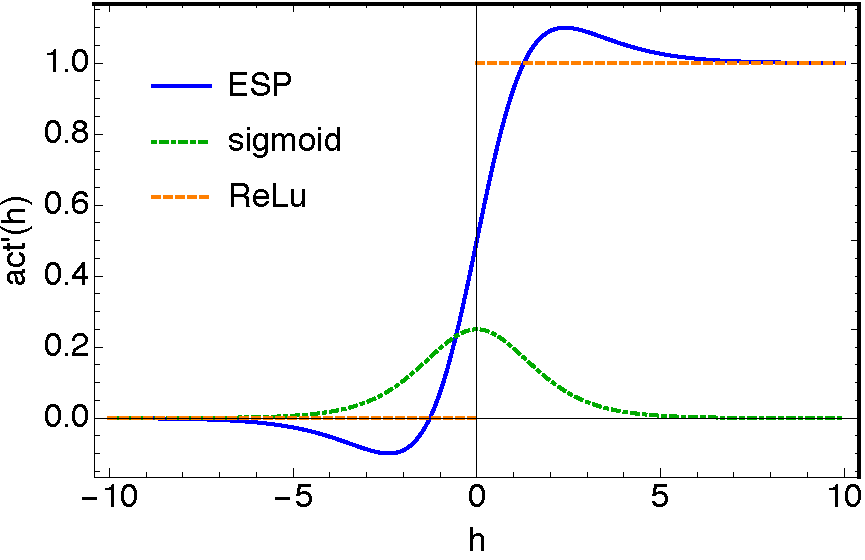
\includegraphics[width=\textwidth]{act.pdf}
        \caption{derivative of the activation}
        \label{fig:gradact}
    \end{subfigure}
    %
\caption{\label{fig:activations} The three activations as a function of $h$ for $\beta=1$. The difference between the {\it sigmoid} (a distribution), {\it ReLU} and {\it Swish} (expectation values) is evident. For $\beta \gg 1$, {\it Swish} tends to {\it ReLU}.  }
\end{figure*}
%

	So far we have discussed the information processing mechanism of a single hidden layer; going back to Eq.~\eqref{eq:chain}, we see that additional hidden layers can be introduced by exploiting the chain rule further. However, there is a final step we need in order to bridge Eq.~\eqref{eq:chain} and Eq.~\eqref{eq:ps5}  or \eqref{eq:ps6}, that is fixing $P(j) \simeq \delta(j- \langle j \rangle)$, i.e. fixing the neuron's output distribution on its first moment. There is no reason {\it a priori}  for this approximation other than computational, and it would be certainly interesting to study how the network's performance and complexity changes when this approximation is relaxed, for example by introducing fluctuations (second moment) in the output signal.


	We would like to conclude this section noticing that in spin glasses~\cite{parisi2, giardina}, the energy landscape presents an increasing number of degenerate local minima as the temperature is lowered, a feature shared with the Hopfield model of associative memory~\cite{amit} and RBM. The effect of noise in FFNs was recently considered in Ref.~\cite{pratik}, where an improved optimization algorithm based on the maximum entropy principle was proposed.
\subsection{Back-propagation: a probabilistic point of view} \label{sub:back}

 %
At the heart of any FFN model is the back propagation algorithm~\cite{hertz, bishop}. Forward propagation returns a first ``guess'' on the value of the learning parameters, that are subsequently adjusted layer by layer by minimizing a properly defined loss function, i.e. the energy of the system. Consider the output layer ``L'', then the gradient of the weights is
%
\begin{align} \label{eq:gradsL}
\frac{\partial \mathscr{L}}{\partial \mathbf{w}_L } &=  \frac{1}{m} \sum_{\mu=1}^m \, \left[ \mathbf{e}^{\mu} \, \mathbf{g}(\hat{\mathbf{h}}^{\mu} _L) \right]  \mathbf{a}_{L-1}  \\ \nonumber
\hat{\mathbf{g}}(\mathbf{h}^{\mu}_l) &=  \boldsymbol{\sigma}(\boldsymbol{\beta}_l \, \hat{\mathbf{h}}^{\mu}_l)[ 1 + \hat{\mathbf{h}}^{\mu}_l \boldsymbol{\beta}_l \, \boldsymbol{\sigma}(-\boldsymbol{\beta}_l \, \hat{\mathbf{h}}^{\mu}_l) ] ,
 \end{align}
%
where $\mathbf{e}^{\mu}$ is the residual error, depending on the difference between the network output $\hat{y}^{\mu} $ and the ground truth vector $y^{\mu}$. In the optimization phase we look for the stationary point  $\partial \mathscr{L}/\partial \boldsymbol{\theta}^{\alpha}_l=0$, where $\boldsymbol{\theta}^{\alpha}_l = \left\{ \mathbf{w}_l, \mathbf{b}_l, \boldsymbol{\beta}_l \right\} $ is the set of learning parameters. For a linear network, this condition is  strictly satisfied if $ \mathbf{e}^{\mu}=0$. However, in a non linear network we can also have $g(\hat{\mathbf{h}}^{\mu})=0$. In principle, there may be situations in which $\mathbf{e}^{\mu}$ is far from zero but $g(\hat{\mathbf{h}}^{\mu}) \simeq 0$, in which case learning will not be effective. For a $\sigma$ activation, $\mathbf{g}(\hat{\mathbf{h}}^{\mu}_l) = \boldsymbol{\sigma}(\boldsymbol{\beta}_l \, \hat{\mathbf{h}}^{\mu}_l)\boldsymbol{\sigma}(-\boldsymbol{\beta}_l \, \hat{\mathbf{h}}^{\mu}_l)$, commonly known in physics as a phase space factor; it appears e.g. in the collision integral of the Boltzmann equation~\cite{roberto}, which describes the transition probability from an occupied to an empty state. Ref.~\cite{tishby1, tishby2} show that there are two distinct phases of learning: empirical error minimization (the residual) and representation learning. Following the discussion of the previous section, we can identify the latter with the task of optimizing $g(\hat{\mathbf{h}}^{\mu})$. When $\hat{h}_i \gg 1/\beta_i$, i.e. when the signal greatly exceeds the noise, then $\sigma( \beta_i \,\hat{ h}_i) \equiv P(s_i=1| \bar{x}_i)  \simeq 1$ \footnote{ Here $\bar{x}_i$ is the input of the unit, not necessarily the input data of the network.} and the back propagated signal is small, being proportional to $g(\hat{h} ) \simeq 0$. We then have the paradoxical situation in which, although the lower dimensional representation of the information is considered to be relevant, learning is likely to be inefficient.

Consider now the same limiting behaviour for {\it Swish}. If $\hat{h}_i \gg 1/\beta_i$ we now have $g(\hat{h}^{\mu}_i)\simeq 1$, i.e. the representation learning phase is completed and learning moves towards minimising the empirical error. In the opposite limit, the signal is much smaller than the noise and learning is impossible, as expected. Finally, in the noiseless case one obtains the {\it ReLU} solution $g(\hat{h}^{\mu}_i) = (1, 0) $, for $\hat{h}_i $ respectively greater or smaller than zero. This corresponds to a purely ``excitatory'' network, in which representation unlearning is not possible. In other words, the fact that {\it Swish} can be negative for $\sigma(\hat{h})/\beta <\hat{h}<0$ allows for greater flexibility and the possibility to avoid plateaus surrounding local minima and saddle-points. In Ref.~\cite{dauphin} it was proposed that plateaus of zero (or small) curvatures in the loss are mostly responsible for slowing down or preventing convergence of gradient descent. These plateaus are a consequence of continuous symmetries in the loss function (Noether's theorem) that are generated, in analogy to the $L^2$ regularization, by the large values for individual variables \cite{energyland}. The following section provides a numerical analysis to support this picture. Details of the the back-propagation algorithm with {\it Swish} for a general $L$ layer network can be found in the SM.
%
\begin{figure*}[t!]
\centering
	\begin{subfigure}[b]{0.48 \textwidth}
	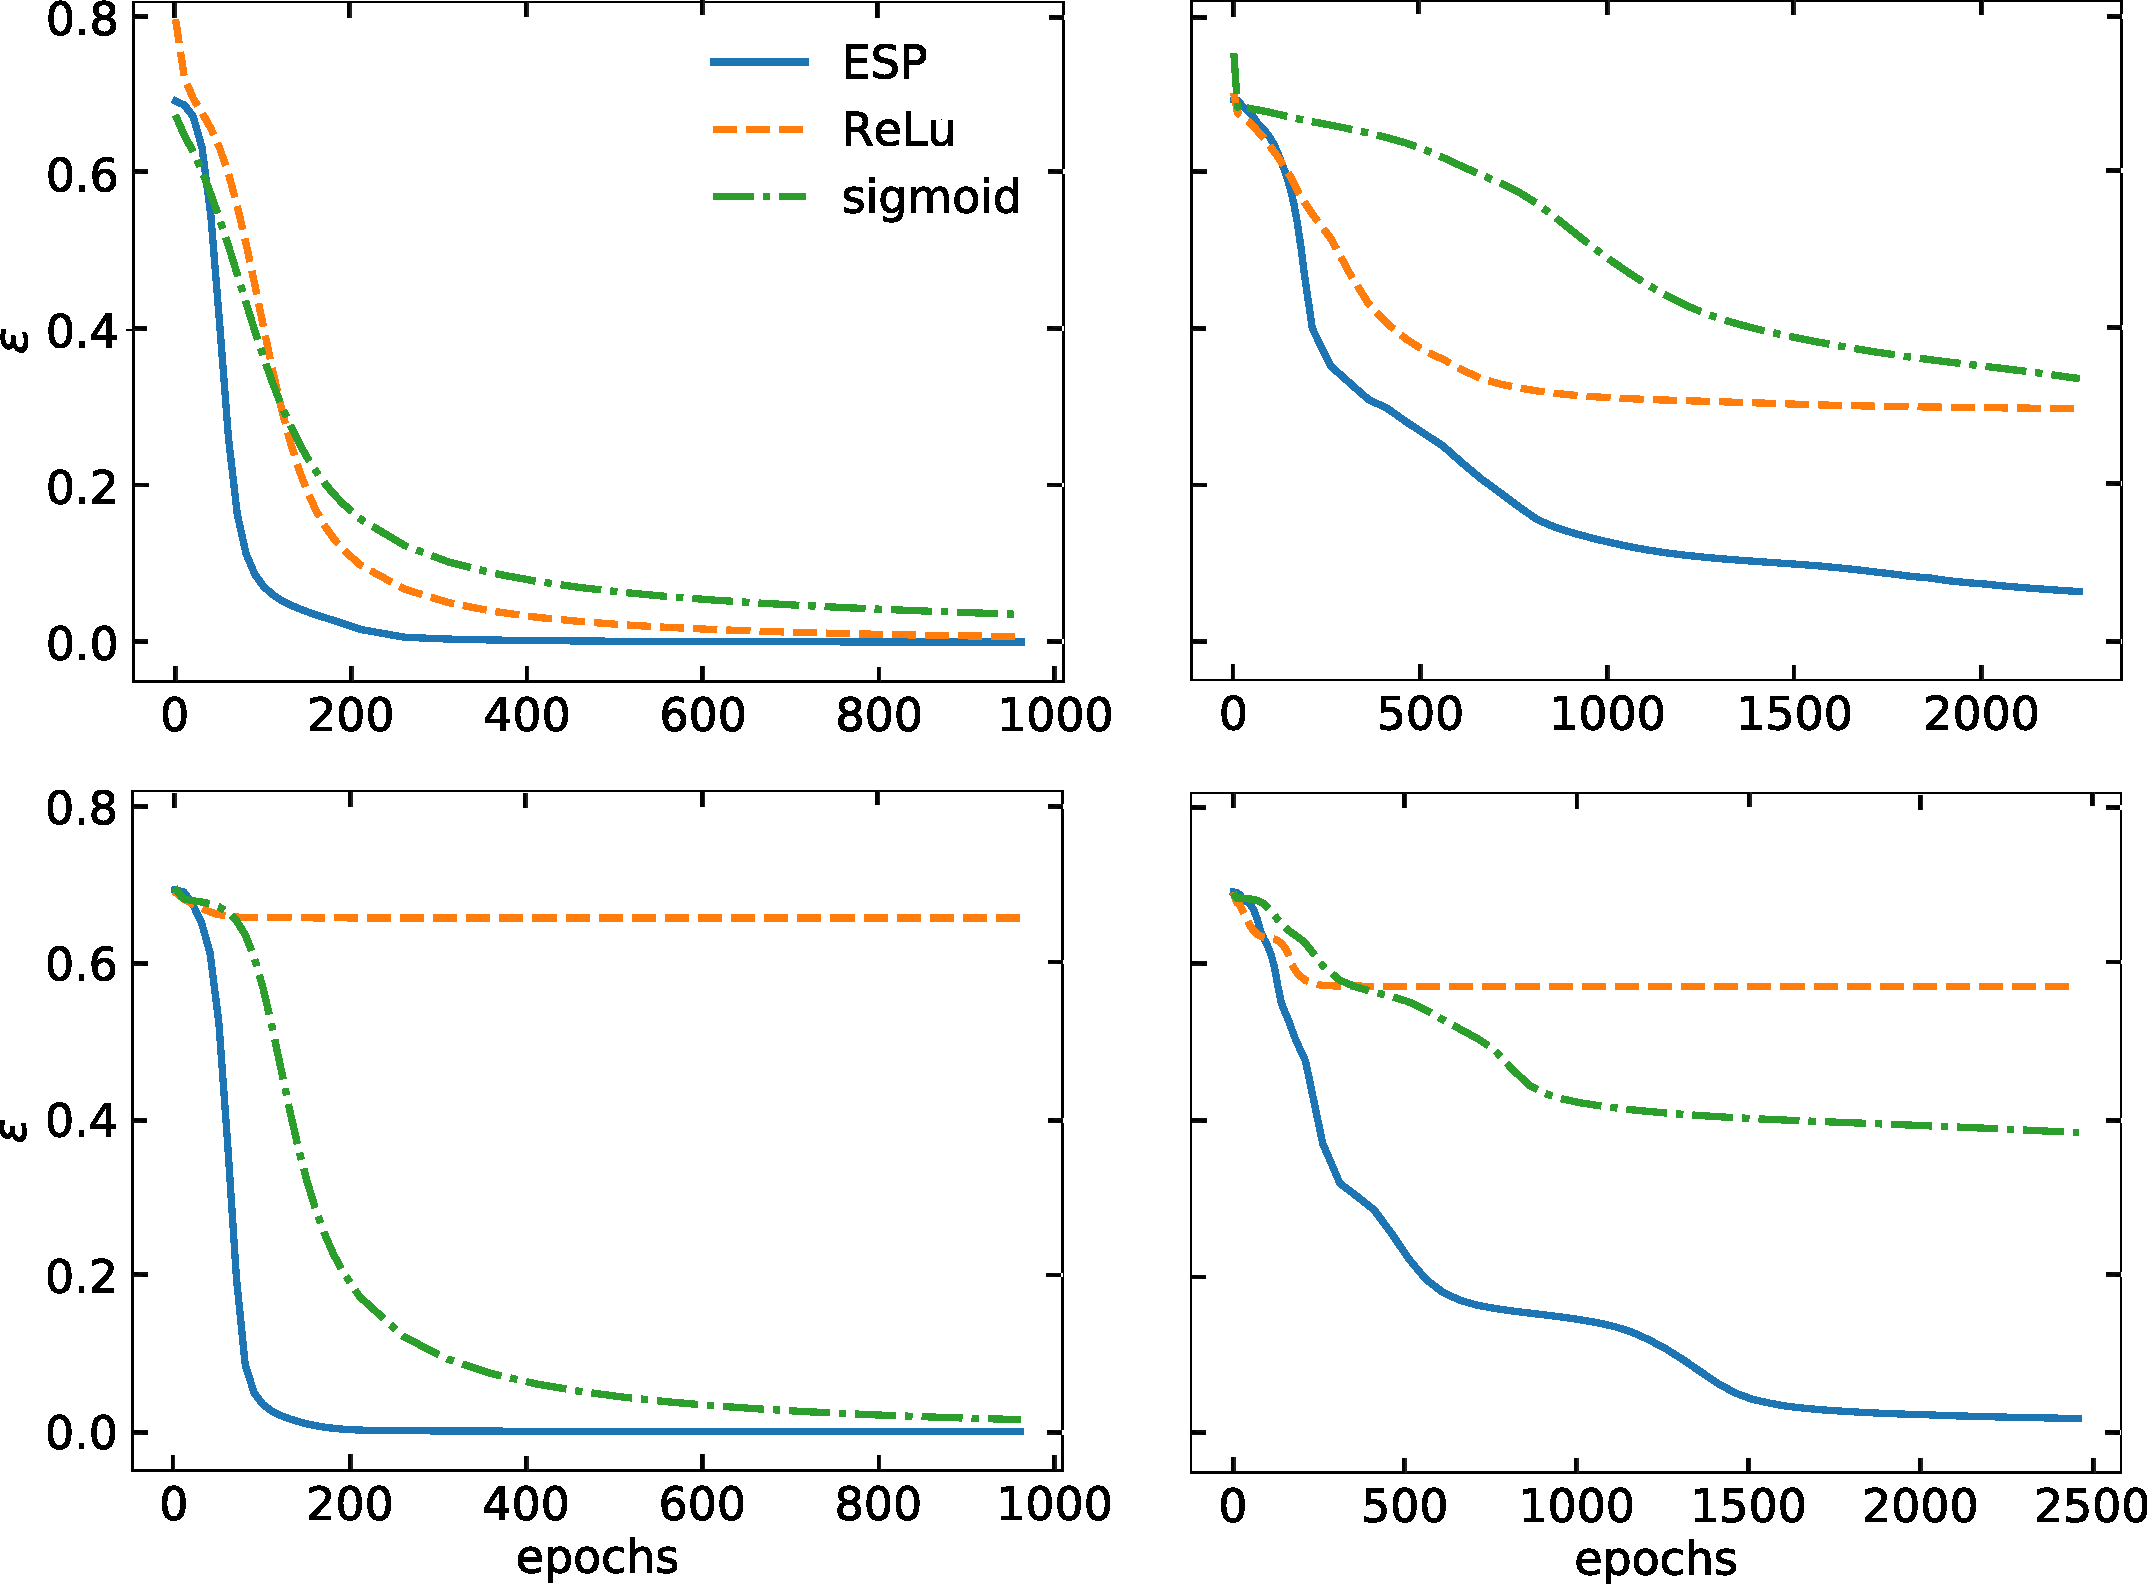
\includegraphics[width = \textwidth]{costs.pdf}
	%\label{fig:cost1}
	\end{subfigure}
 	~
	\begin{subfigure}[b]{0.48 \textwidth}
 		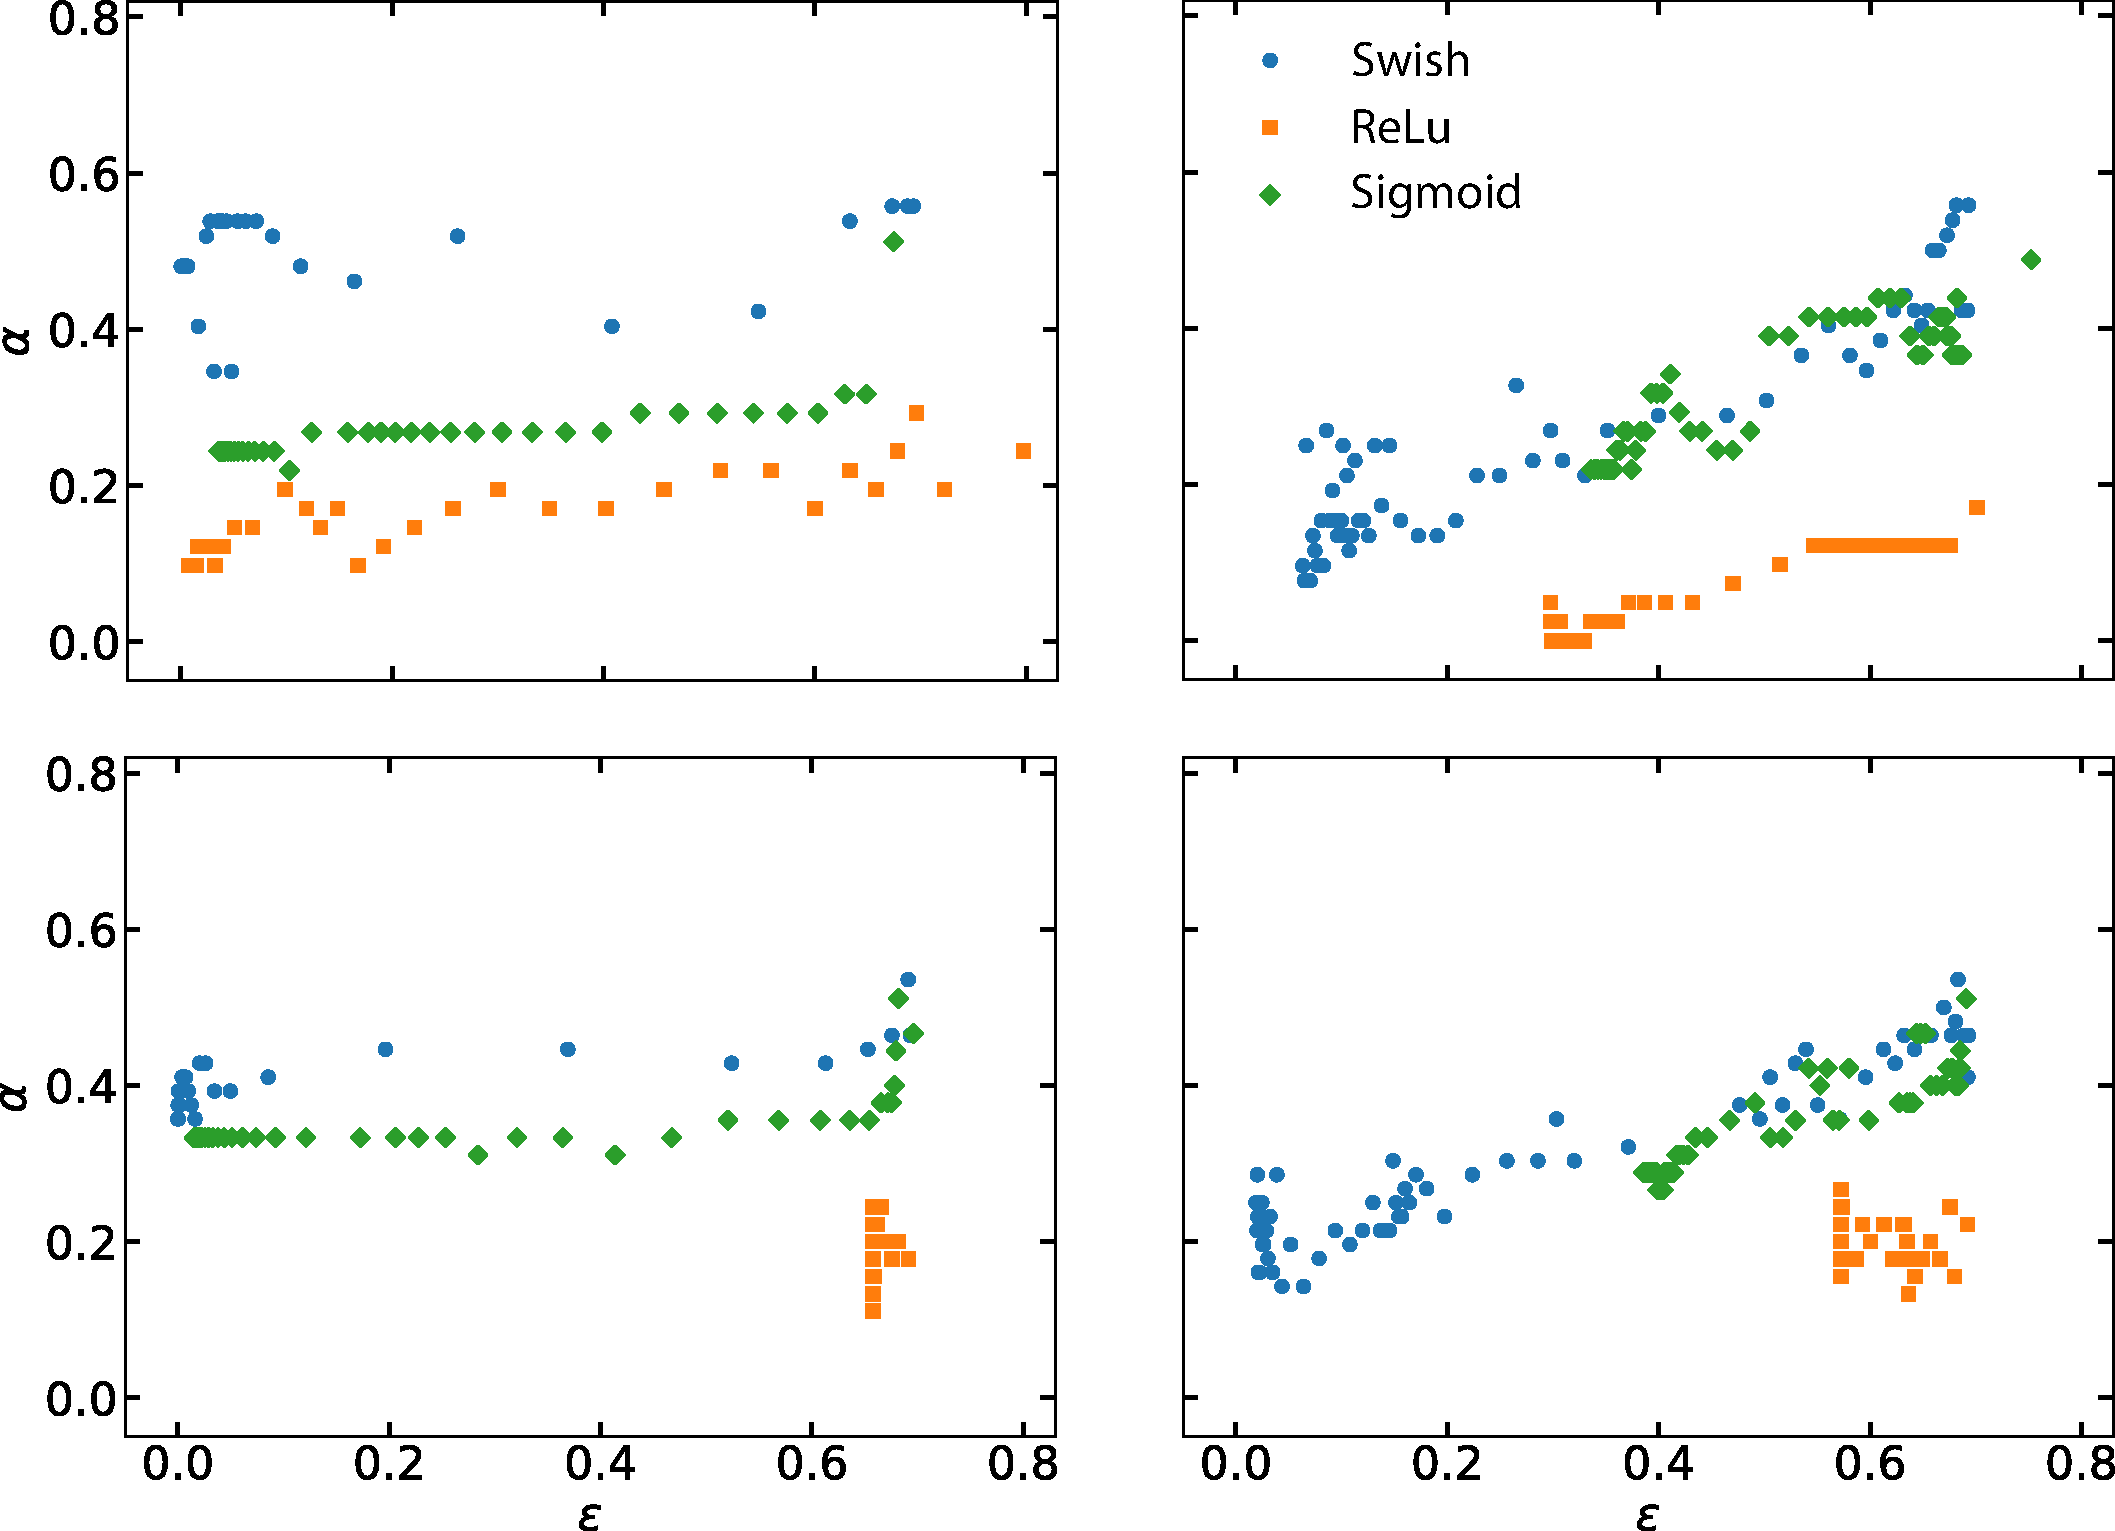
\includegraphics[width = \textwidth]{alpha.pdf}
		%\label{fig:index1}
	\end{subfigure}
	%
	\caption{ \label{fig:index} (a) Loss functions for linear (left) and non-linear (right) binary classification. (Top) 10 units hidden layer (Bottom) two hidden layer of 8 and 2 units respectively. All cases have a sigmoid activation in the last layer and a learning rate of 0.01. (b) $\alpha$ index  v.s. energy for the single layer network with linear (left) and non-linear (right) decision boundary. Curves are evaluated with the same number of epochs: 1000 (left) and 2300 (right). }
\end{figure*}
 %
\section{Numerical Analysis}
%
A thorough performance analysis of {\it Swish} versus other popular choices of activations was carried out in Ref.~\cite{prajit}, where it was shown that the former outperformed all other choices on image classification tasks using a convolutional structure. It was also noted that to take full advantage of {\it Swish} one should also reconsider the way convolution is performed; for the moment, we leave this interesting point open and rather focus on understanding the optimization dynamics in pure FFNs.  We have considered both artificial and experimental datasets trained with ADAM gradient descent~\cite{adam}. Given that both datasets lead to the same qualitative features, we focus our analysis on the former and discuss the latter, together with additional details in the SM.

In Fig.~\eqref{fig:index}(a) we show the loss functions for two binary classification tasks: a linear and a non-linear one, each trained with one and two hidden layers. For the linear task with a single, 10 units layer (adding more units does not improve performance), all three activations attain full train/test accuracy but {\it Swish} is the fastest converging.  For the non-linear task, {\it ReLU} quickly converges to a suboptimal plateau. To obtain a better understanding, we have evaluated two different indices: the fraction of negative eigenvalues of the Hessian --$\alpha$--(Fig.~\ref{fig:index}(b) )and the fraction of zero eigenvalues -- $\gamma$ --  (Fig.~\ref{fig:res}(b) ). The former measures the ratio of descent to ascent directions on the energy landscape; when $\alpha$ is large, gradient descent can quickly escape a critical point -- a saddle point in this case --  due to the existence of multiple unstable directions. However, when a critical point exhibits multiple near-zero eigenvalues, roughly captured by $\gamma$, the energy landscape in this neighborhood consists of several near-flat (to second-order) directions; in this situation, gradient descent will slowly decrease the training loss. In Ref.~\cite{dauphin} it was noted that energy plateaus are responsible for slowing down or preventing learning. This can be understood by considering the case in which learning completely fails: the loss does not decrease and all the eigenvalues of the Hessian are zero. Noether's theorem infers that these eigenvalues are originated by symmetries of the loss function. %In this case the analysis is not conclusive and higher order inspection is needed to reveal possible inflection points.
In general, we find that  for {\it ReLU} networks $\gamma \neq 0$, while this is typically not the case for both {\it Swish} and sigmoid-networks. Taking the two layer case as a representative example, we show that {\it ReLU} networks are sensitive to fine tuning of the model: choosing a $10-2$ or a $8-5$ configuration over the $8-2$ considered here, greatly improves learning. In stark contrast, {\it Swish} networks exhibit consistent performance over a wider choice of architecture/learning parameters. Although the performance impact might be fairly small for small networks, it certainly plays an important role for larger datasets, as discussed in Ref.~\cite{prajit}.
In Fig.~\eqref{fig:index} we show the $\alpha$ index, usually smaller for the {\it ReLU} network, and a finite value of $\gamma$ that slows down learning. We find $\gamma \simeq 0.45-0.6$ for {\it ReLU} and $\gamma=0$ for {\it Swish} and $\sigma$, both for the linear and non-linear task. We have also evaluated the fraction of residuals $e^{\mu} \simeq (\hat{y}^{\mu} - y^{\mu})/m$ closer to zero and found, surprisingly, that {\it Swish} greatly outperforms the other activations in minimizing the empirical error, see Fig.~\eqref{fig:res}.
%
 In addition, we find that the eigenvalue distribution obtained with {\it ReLU}  {\it shrinks} with increasing training epochs, giving rise to the singular distribution reported in Ref.~\cite{penn1, levent}. In contrast,{\it Swish} show a significantly wider spread in the eigenvalue distribution at the end of training, see SM for details and discussions, together with results for the MNIST dataset.

  {\it Swish} training networks can break the symmetries of the loss function and reach extremal points that have higher number of zero residuals (in Physical terms, lower energy minima).
  This is obtained by preventing large values of the individual components in the Hessian eigenvectors-variables transformation matrices at the minima. In Fig.( \ref{fig:eigvect} ) , the Hessian eigenvectors vs the individual variables are plotted in the case of Relu, Sigmoid and Swish networks (see the linear binary classification with two 8-2 hidden layer of 8 and 2 units Fig. ~\eqref{fig:index} bottom left loss function minimization). In the case of Relu, the loss function minimization is almost immediately reached after 300 epocs. This is reflected in the Hessian eigenvectors that still coincide with the variables (in the Figure, the bar indicate the coefficient value of the eigenvectors). In the Sigmoid case, the Hessian eigenvectors are spread more uniformly on the variables showing a sort of graining regularization with respect to the Relu case. Nevertheless, there is still a concentration of high value Hessian coefficients in two sub-matrices. Lastly, in the Swish case, the Hessian coefficients are spread almost uniformly over the transformation matrix. We stress that this effect has some analogies with the regularization that prevents overfitting disfavouring large values for individual variables.
  In Fig. ( \ref{fig:eigvect2} ), the same analysis is repeated for the non-linear two hidden 8-2 layer network. Whereas in the Relu results still show a localization of variables in the eigenvectors, in the Sigmoid and Swish case the Hessian eigenvectors involve a broader number of variables. Nevertheless, in the Swish case, the number of large value coefficients is still less than in the Sigmoid case.
%
\begin{figure*}[t!]
 \centering
 	\begin{subfigure}[b]{0.48\textwidth}
 	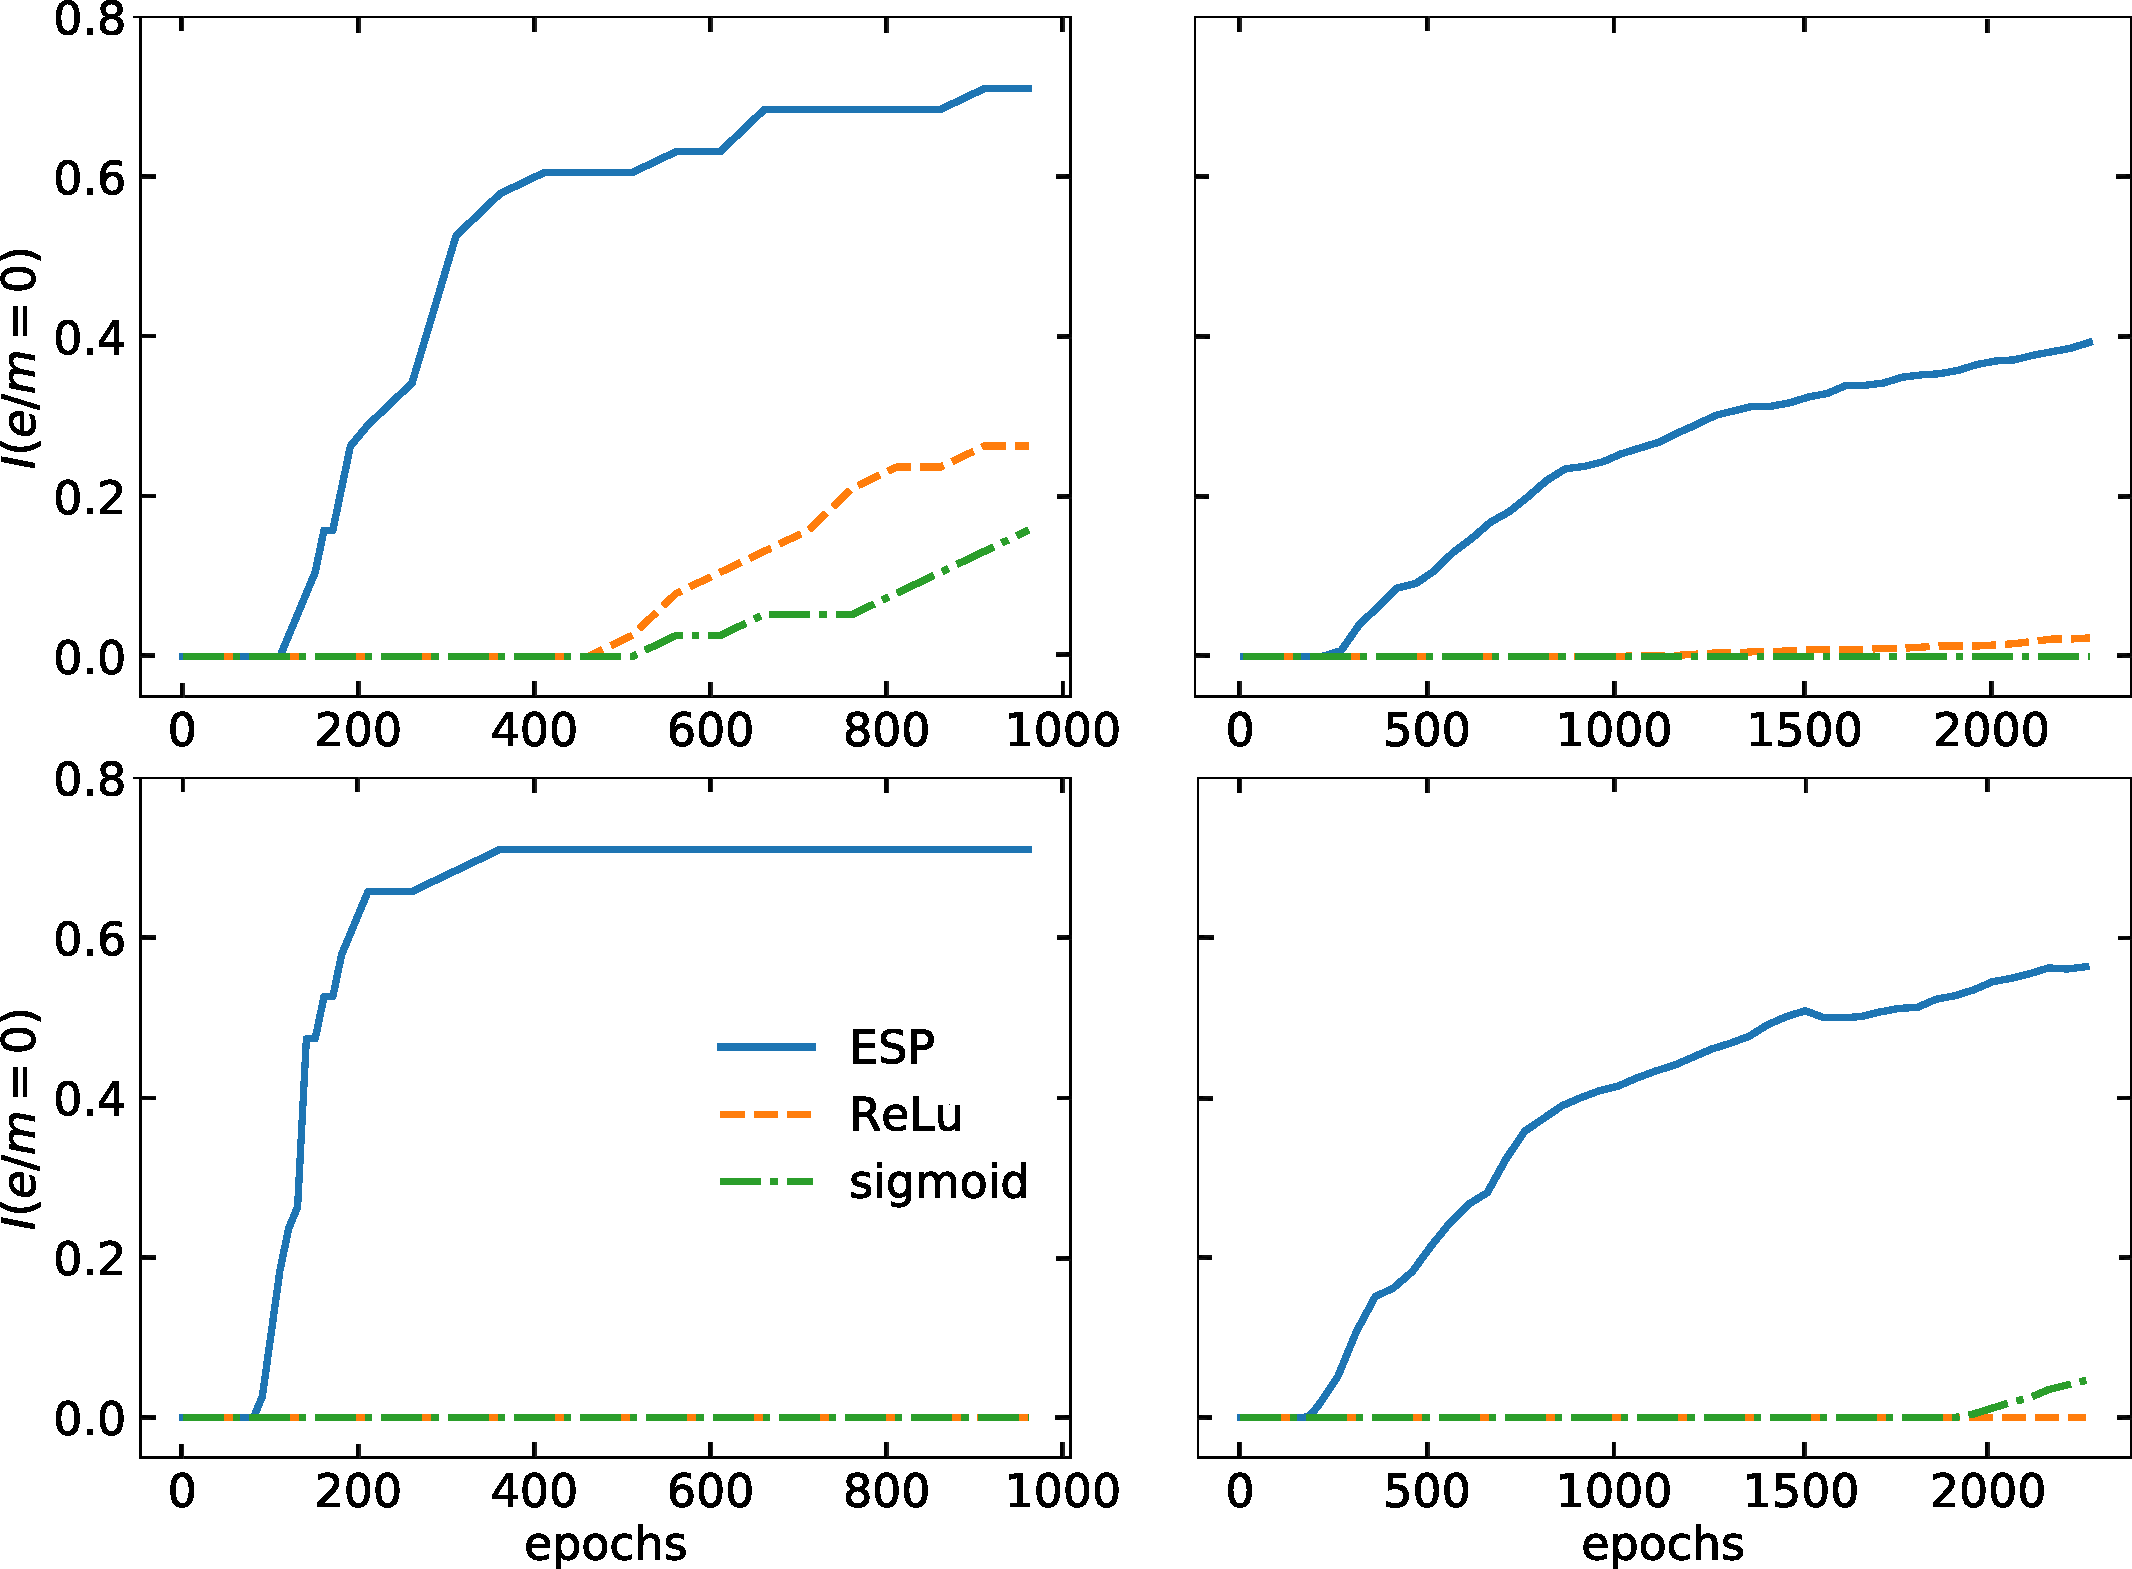
\includegraphics[width=\textwidth]{residues.pdf}
	\label{fig:res}
	\end{subfigure}
	~
	\begin{subfigure}[b]{0.48\textwidth}
 	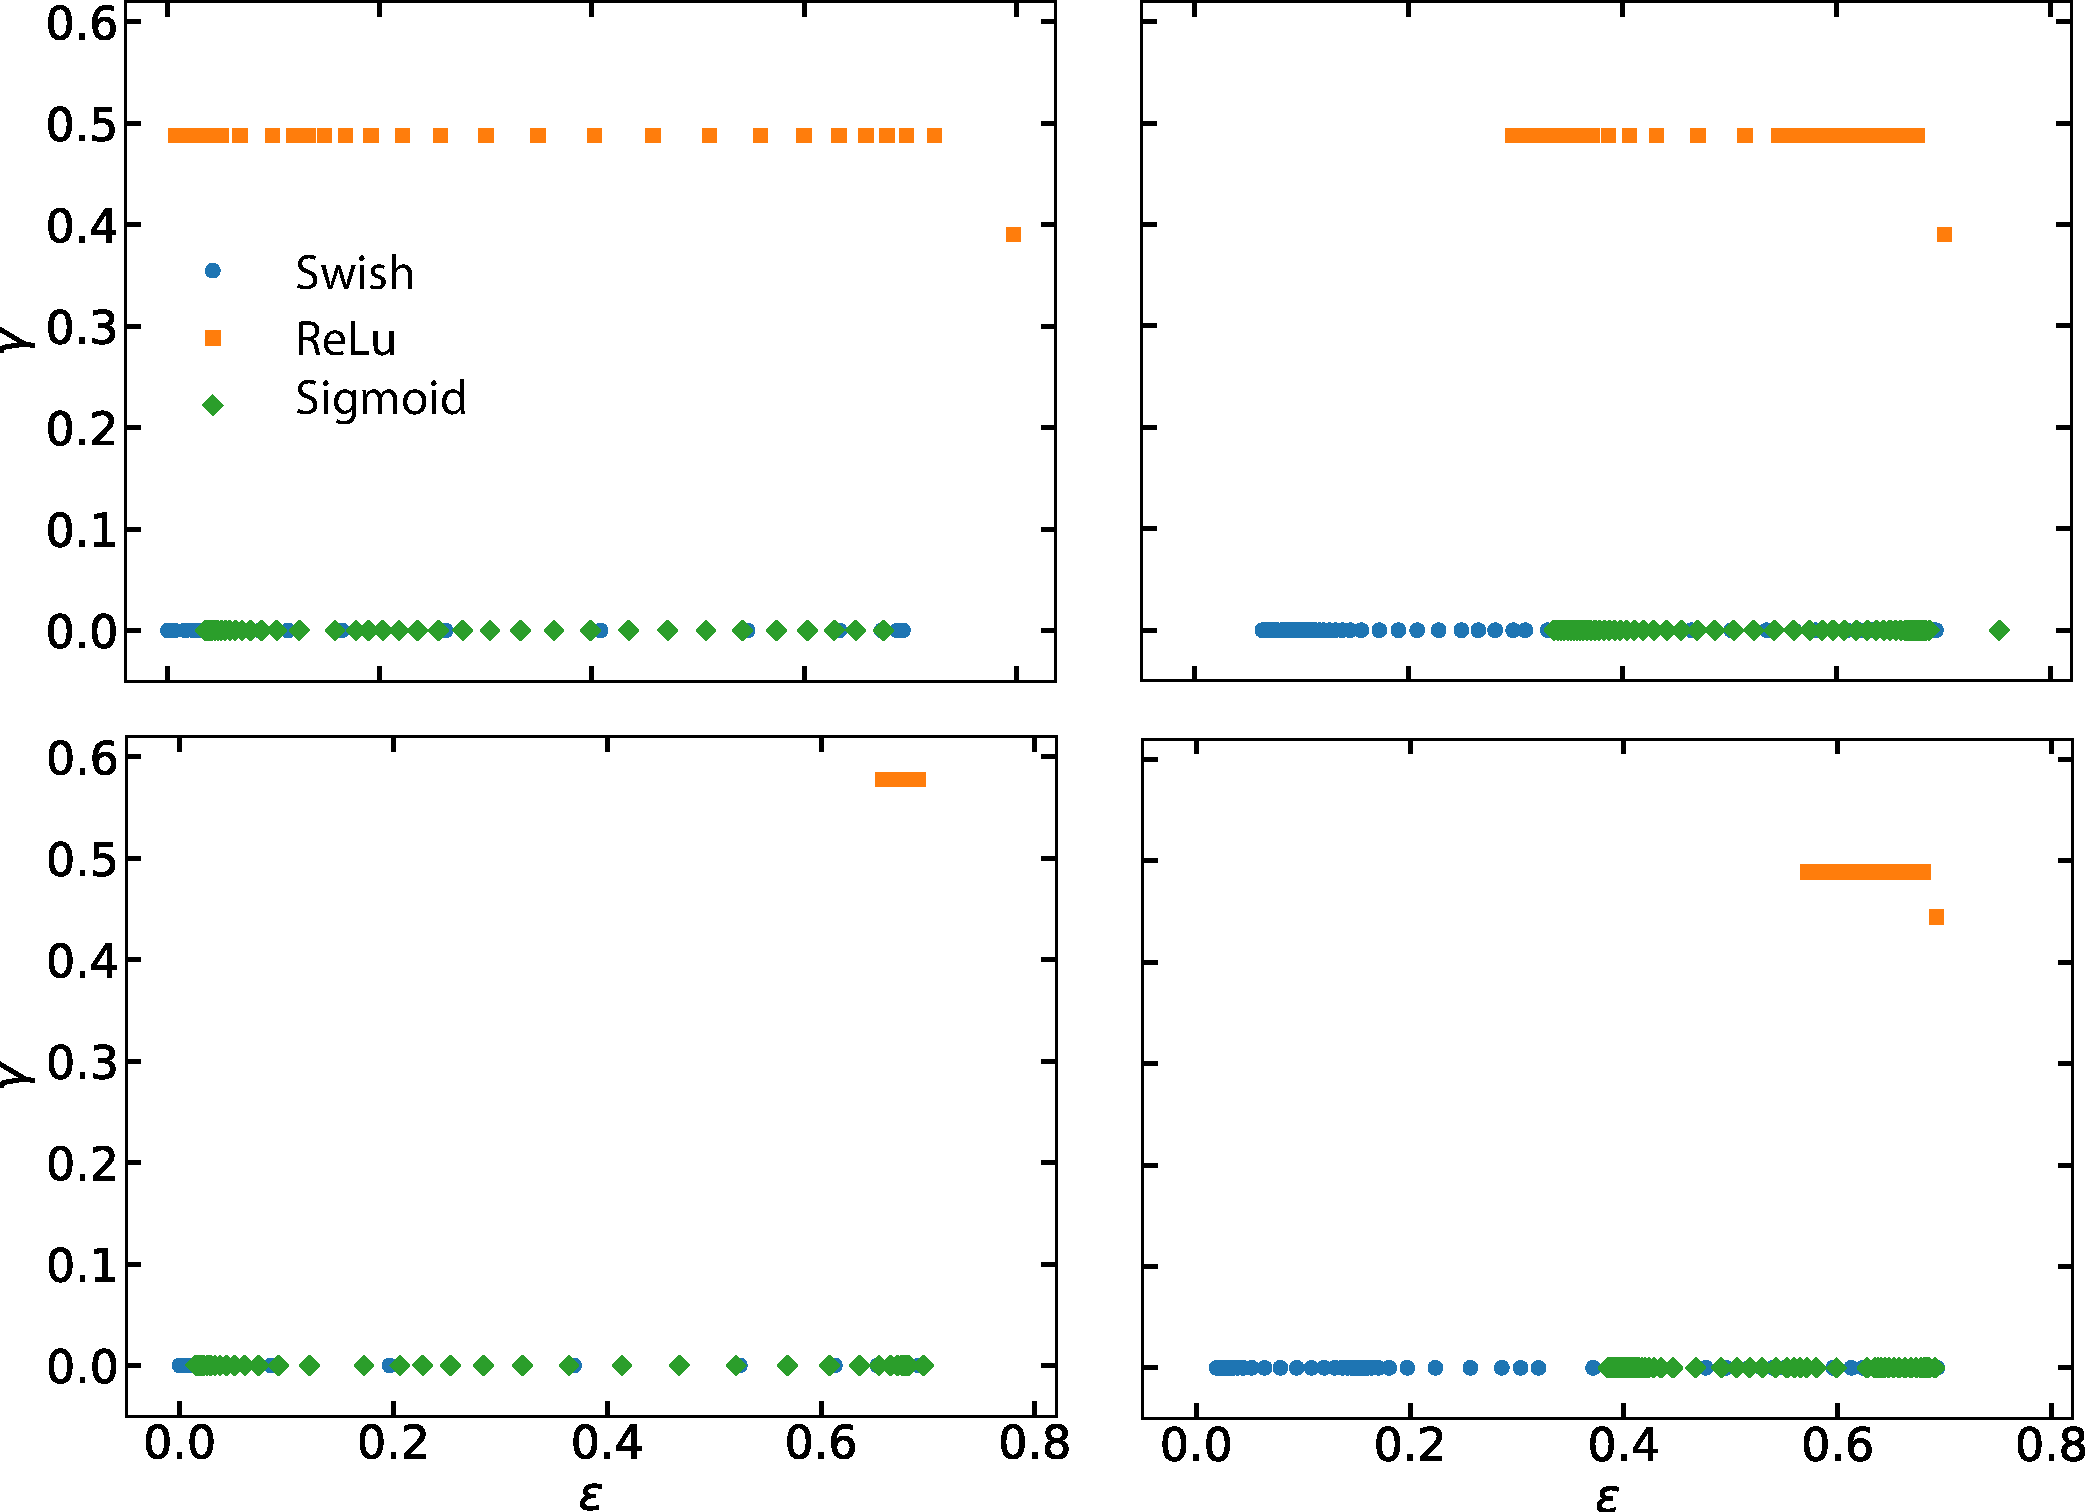
\includegraphics[width=\textwidth]{gamma.pdf}
	\label{fig:gamma}
	\end{subfigure}
	 %
\caption{ \label{fig:res}  Fraction of zero residuals as a function of training epochs for the single 8-2 layer network with linear (top/bottom left) and non-linear (top/bottom right) decision boundary. (right) Fraction of zero eigenvalues. (Top left/right) linear/non-linear dataset with a single, 10 units hidden layer. (Bottom left/right)  linear/non-linear dataset with two hidden layers of 8 and 2 units respectively. }
\end{figure*}
%

\begin{figure*}[t!]
	\centering
		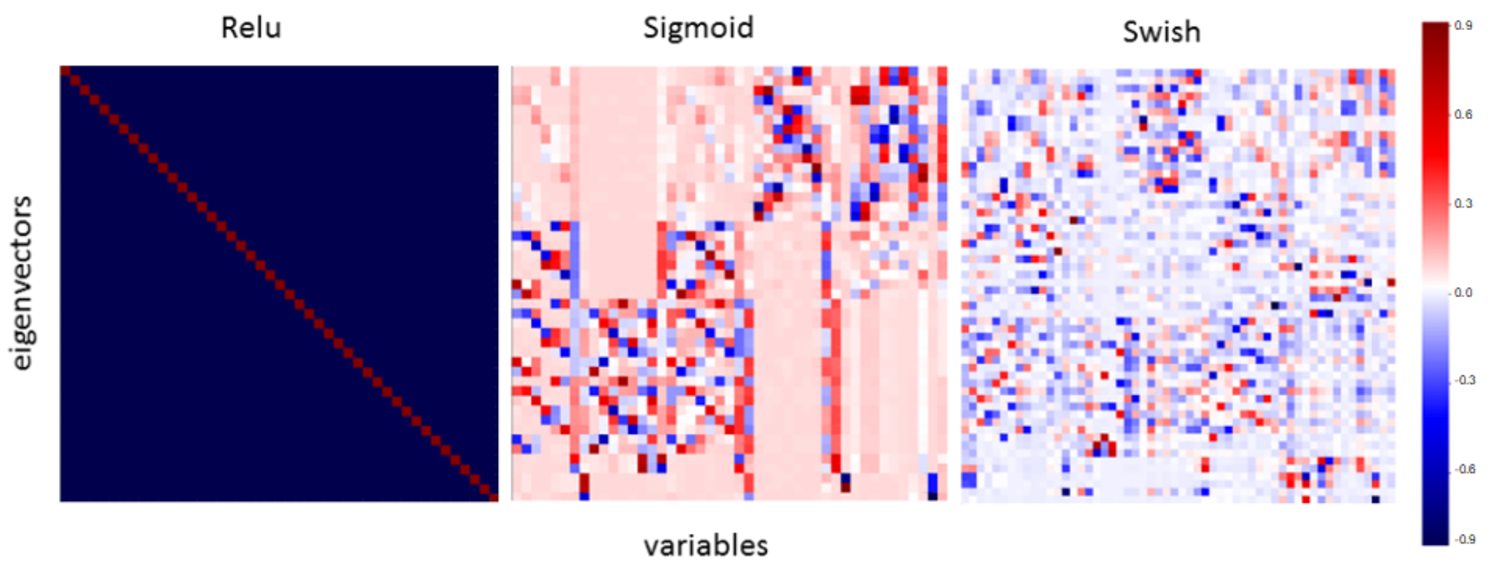
\includegraphics[width=\textwidth]{eigen_lin.pdf}

\caption{  \label{fig:eigvect} Hessian eigenvectors (column) variables (row) for the linear two hidden layer of 8 and units for Relu, Sigmoid and Swish. the bar indicates the value of the eigenvector coefficients.}
\end{figure*}

\begin{figure*}[t!]
	\centering
	\includegraphics[width=\textwidth]{eigen_nlin.pdf}

	\caption{  \label{fig:eigvect2}(left) Hessian eigenvectors (column) variables (row) for the non-linear two hidden layer of 8 and units for Relu, Sigmoid and Swish. the bar indicates the value of the eigenvector coefficients.}
\end{figure*}
\section{Conclusions and perspectives}
%
In this work we have introduced an energy-based model that allows systematic construction and analysis of FFNs. It provides a  coherent interpretation of the computational process of each and every unit (neuron). Furthermore, it presents a method that overcomes the dimensional mismatch that arises from using heuristic activations. Enforcing dimensional consistency naturally leads to a class of activations with the prime focus of propagating the expectation value of processed signals. Our results provide a theoretical justification of the \textit{Swish} activation found in Ref.~\cite{prajit}. In addition, we demonstrate the superiority of this {\it Swish} activation through numerical experiments that reveal the geometry of its loss manifold. {\it ReLU} networks, unlike $\sigma$ and $tanh$,  do not suffer from dimensional mismatch, yet their restricted phase space results in a finite fraction of null directions of gradient descent that can slow down or, in some cases, completely prevent learning. To overcome this problem, one needs a detailed fine tuning of the network's topology that likely increases the complexity of the learning task. In stark contrast, {\it Swish} trained networks are less prone to fine tuning and outperform other activations on minimizing the empirical error. We hope this statistical mechanics view can facilitate future studies of FFNs, e.g. to explore the scaling relation between the {\it Swish} Hessian's eigenvalue distributions and the parameters that describe its loss landscape, analogous to those studied in Ref.~\cite{penn1} for standard activations. As previously discussed, the Renormalization Group (RG) approach could hint at designing principles of FFNs, as it delineates how complex behavior emerges from the elementary constituents of a system. Although this framework has been considered in Ref.~\cite{mehta, maciej}, the complete mathematical formalism to correctly use it in FFNs is still missing. We believe this could answer some of the most pressing questions in the construction of FFNs, namely: given a dataset showing specific strength and extent of input/output correlations, what is the optimal network topology? Finally, extensions of the methods discussed here to Convolutional and Recurrent architectures could lead to substantial performance improvement and, potentially, faster training algorithms.



\section{Acknowledgements}

M.M. would like to thank Ned Phillips, Bill Phillips, Sarah Chan and Roberto Raimondi for support and discussions. A special thanks to  F\'abio Hip\'olito and Aki Ranin for carefully reading and commenting the manuscript. T.C. would like thank Shaowei Lin for useful discussions and for financial support from the startup research grant
SRES15111, and the SUTD-ZJU collaboration research\\
grant ZJURP1600103. P.E.T would like to thank M. D. Costa for help with HPC. Some of the calculations were carried out at the HPC facilities of the NUS Centre for Advanced 2D materials. Finally, M.M. And T.C. would like to thank the AI Saturday meetup initiative organised by Nurture.ai, that sparked some of the ideas presented in this work.

\appendix
\section{Cross Entropy Loss} \label{a:loss}
%
In this appendix we present a derivation of the cross entropy loss function using large deviation methods~\cite{mezard}. A useful starting point is the definition of the accuracy of a classification task, that is the number of times the network prediction $\hat{y}$ equals the provided solution $y$. This corresponds to the conditional probability $P(y|\hat{y}) =  \mathbb{I}(y = \hat{y})$ in Eq.~\eqref{eq:chain}.  As $\hat{y}$ is a random variable, we want to know which is the probability of obtaining the true value $y$ in a series of ``experiments'' in which $\hat{y}$  has a certain probability to be equal to $y$. According to Eq.~\eqref{eq:chain}, and using the standard definition  relating the Loss function to the log-probability $\mathscr{L} = - \log P(\mathbf{y})$, we need to evaluate
%
 \begin{align} \label{eq:cl1}
-\log P(\mathbf{y}) = - \log \int d \hat{\mathbf{y}}\, P(\mathbf{y} | \hat{\mathbf{y}}) \, P(\hat{\mathbf{y}}),
 \end{align}
%
From a physics perspective, the above expression corresponds to an {\it annealed } average~\cite{parisi2, giardina} and we will discuss its meaning at the end of the calculation. For the moment, we assume that we can replace $y \to y^{\mu}$ and $\hat{y} \to \hat{y}^{\mu}$ directly in Eq.~\eqref{eq:cl1}, i.e. we fix the random variables on the observed data. Using the Dirac delta  as a representation of the Indicator function we have
%
 \begin{align} \label{eq:cl1}
 P(y) & =  \int  \left( \prod_{\mu} d \hat{y}^{\mu} \right)  \,  \prod_{\mu} \delta( y^{\mu} - \hat{y}^{\mu})  \, P(\hat{y})\\ \nonumber
 &=  \int  \left( \prod_{\mu}  \frac{d\lambda^{\mu}}{2\pi} \right) \prod_{\mu}  e^{i \, \sum_{\mu} \lambda^{\mu} \, y^{\mu} } \chi(\lambda^{\mu}).
  \end{align}
%
where we have introduced $m$ Lagrange multipliers $\lambda$ to enforce the $\delta$-function constraint and identified  the characteristic function
%
\begin{align} \label{eq:char}
 \chi(\lambda^{\mu}) &=  \int  \left( \prod_{\mu} d\hat{y}^{\mu} \right)  P(\hat{y}^{\mu} )  \, e^{-i \sum_{\mu} \lambda^{\mu} \, \hat{y}^{\mu}}
 \end{align}
%
Let us consider the case of i.i.d. examples, distributed according to the Bernoulli distribution:
%
\begin{equation} \label{eq:bern}
P(\hat{y}^{\mu} ) = \int d\boldsymbol{\theta} \left\{ q^{\mu}(\boldsymbol{\theta}) \, \delta(\hat{y}^{\mu}-1 ) + (1-q^{\mu}(\boldsymbol{\theta}) ) \, \delta(\hat{y}^{\mu}) \right\},
\end{equation}
%
where each outcome is either $1$ or $0$ with a {\it sample dependent} probability $q^{\mu}(\boldsymbol{\theta})$ being the output value of a Neural Network solving a binary classification task; as such, $q$ has the functional form of a sigmoid function with $\boldsymbol{\theta}$ a set of network parameters. In this case, Eq.~\eqref{eq:char} reads
 %
\begin{align} \label{eq:char}
 \chi(\lambda^{\mu}) &=  \int  d\boldsymbol{\theta} \left[ q^{\mu}(\boldsymbol{\theta} ) e^{-i \, \lambda^{\mu} } +(1-q^{\mu}(\boldsymbol{\theta} )) \right].
 \end{align}
%
Using this expression back in Eq.~\eqref{eq:bern} we arrive at the intermediate result
%
 \begin{align} \label{eq:cl2}
 P(y) &= \int d\boldsymbol{\theta} \int  \left( \prod_{\mu}  \frac{d\lambda^{\mu}}{2\pi} \right) e^{i \, \sum_{\mu} \lambda^{\mu} \, y^{\mu} +\sum_{\mu} \log \left[ q^{\mu} e^{-i \, \lambda^{\mu} } +(1-q^{\mu}) \right] }  \\ \nonumber
 &=  \int  \left( \prod_{\mu}  \frac{d\lambda^{\mu}}{2\pi} \right) e^{m \, S[\lambda]}.
 \end{align}
%
For a large number of training examples $m$, we can solve the above integral using the steepest descent, i.e. using a maximum likelihood approach. This fixes the value of the Lagrange multipliers:
%
\begin{align} \label{eq:cl3}
\frac{\partial S[\lambda]}{\partial \lambda^{\mu}} &= i \, y^{\mu} - \frac{i \, q^{\mu} \, e^{-i \, \lambda^{\mu}}}{q^{\mu} \, e^{-i \, \lambda^{\mu}} + (1-q^{\mu})} = 0 \\ \nonumber
&\rightarrow - i \lambda^{\mu}_{c} =  \log \frac{y^{\mu}(1-q^{\mu}) }{q^{\mu}(1- y^{\mu})}
\end{align}
%
Using the optima back in Eq.~\eqref{eq:cl2} we arrive after some simple algebra to the expression for the cross-entropy:
%
\begin{align} \label{eq:cl3}
P(y) &\simeq \int d\boldsymbol{\theta} \, e^{m S[\lambda_c, \boldsymbol{\theta}]} \\ \nonumber
S[\lambda_c] &= \frac{1}{m} \sum_{\mu} \left\{ y^{\mu} \, \log [ q^{\mu}( \boldsymbol{\theta} ) ] + (1-y^{\mu}) \, \log [1-q^{\mu}( \boldsymbol{\theta}) ] \right\},
\end{align}
%
up to an additive constant depending only on $y$. The final step consists in evaluating the $\theta$ integral again for $m \gg 1$, and take the maximum likelihood value $\theta^*$. Before concluding, it is interesting to draw some parallels with the physics of disordered systems.



\section*{References}

\bibliography{esp}

\end{document}
